%% 
%% Copyright 2007, 2008, 2009 Elsevier Ltd
%% 
%% This file is part of the 'Elsarticle Bundle'.
%% ---------------------------------------------
%% 
%% It may be distributed under the conditions of the LaTeX Project Public
%% License, either version 1.2 of this license or (at your option) any
%% later version.  The latest version of this license is in
%%    http://www.latex-project.org/lppl.txt
%% and version 1.2 or later is part of all distributions of LaTeX
%% version 1999/12/01 or later.
%% 
%% The list of all files belonging to the 'Elsarticle Bundle' is
%% given in the file `manifest.txt'.
%% 
%% Template article for Elsevier's document class `elsarticle'
%% with harvard style bibliographic references
%% SP 2008/03/01

%\documentclass[preprint,12pt,authoryear]{elsarticle}  %default in the template
%\documentclass[preprint,10pt,authoryear]{elsarticle}

%% Use the option review to obtain double line spacing
%% \documentclass[authoryear,preprint,review,12pt]{elsarticle}

%% Use the options 1p,twocolumn; 3p; 3p,twocolumn; 5p; or 5p,twocolumn
%% for a journal layout:
% \documentclass[final,1p,times,authoryear]{elsarticle}
%% \documentclass[final,1p,times,twocolumn,authoryear]{elsarticle}
 \documentclass[final,3p,times,authoryear]{elsarticle}
%% \documentclass[final,3p,times,twocolumn,authoryear]{elsarticle}
%% \documentclass[final,5p,times,authoryear]{elsarticle}
%% \documentclass[final,5p,times,twocolumn,authoryear]{elsarticle}

%% For including figures, graphicx.sty has been loaded in
%% elsarticle.cls. If you prefer to use the old commands
%% please give \usepackage{epsfig}

%% The amssymb package provides various useful mathematical symbols
\usepackage{amssymb}
%% The amsthm package provides extended theorem environments
\usepackage{amsthm}
\usepackage{amsmath}
\usepackage{color, colortbl}
\usepackage{amsmath}
\usepackage{siunitx}
\usepackage{tabularx}
\usepackage[]{algorithm2e}
\usepackage{soul}
\usepackage{glossaries}
\usepackage{subfig}
\usepackage{scalerel}
\usepackage{ulem}
\usepackage{multirow}
\usepackage{tablefootnote}

%track changes on
%\newcommand{\add}[1]{\textcolor{blue}{#1}}
%\newcommand{\remove}[1]{\textcolor{red}{\st{#1}}}
%track changes off
\newcommand{\add}[1]{\textcolor{black}{#1}}
\newcommand{\remove}[1]{\textcolor{red}{\st{}}}


\definecolor{light-gray}{gray}{0.9}


\newcommand{\beginsupplement}{%
        \setcounter{table}{0}
        \renewcommand{\thetable}{S\arabic{table}}%
        \setcounter{figure}{0}
        \renewcommand{\thefigure}{S\arabic{figure}}%
     }


\DeclareRobustCommand{\hlgreen}[1]{{\sethlcolor{green}\hl{#1}}}

\journal{Urban Climate}
\makeglossaries


\begin{document}


\title{Pavement watering as an urban heat mitigation technique}

\author[monash]{Ellie Traill}
\author[melb]{Kerry~A.~Nice\corref{cor1}}
\cortext[cor1]{Principal corresponding author}
\ead{kerry.nice@unimelb.edu.au}

\author[monash]{Nigel Tapper}
\author[monash]{Julie Arblaster}

\address[melb]{Transport, Health, and Urban Design Research Lab, Faculty of Architecture, Building, and Planning, University of Melbourne, VIC, Australia.}
\address[monash]{School of Earth, Atmosphere and Environment, Monash University, Clayton, VIC 3800, Australia.}




\begin{abstract}

Climate change, rapid urbanisation, and ageing populations are reinforcing the need for urban heat mitigation techniques. Pavement watering is one such technique, where evaporative cooling is induced through wetting urban surfaces. The aim of this research is to assess the potential cooling benefits of pavement watering. To do this, a 10$\times$10m section of a car park was watered, and experiments were conducted at midday, the afternoon, and the evening across three days. Pavement watering was found to induce a mean cooling of up to 0.6$^{\circ}$C in air temperature and 2$^{\circ}$C in \gls{utci} at 1.5m. Benefits were related to prevailing conditions, with lower wind speeds associated with greater cooling. Surface temperature was also found to decrease by up to 9.0$^{\circ}$C, and the surface energy balance of the watered carpark was characteristic of a highly evaporative surface. However, there were limitations of the experiments; notably, the assumptions made to correct observations increased uncertainty, and the small scale of the experiment likely limited the observed cooling benefits. Despite this, pavement watering was shown to reduce air temperature and surface temperature, as well as improve thermal comfort, and thus may potentially be used in emergencies to provide cooling in urban areas.

\end{abstract}

\begin{keyword}
Urban climate\sep
urban heat island\sep 
heat mitigation\sep 
pavement watering\sep 
thermal comfort
\end{keyword}



\maketitle

\section{Introduction}\label{sec:introduction}

Urban areas are especially vulnerable to heat facing future trends of increased heatwave frequency and duration \citep{Cowan2014,Perkins-Kirkpatrick2020} driven by climate change \citep{IPCC2022}. In many urban areas in the world extreme heat is the most dangerous natural hazard, including Australia \citep{Coates2014} and Europe \citep{Forzieri2017}, driving higher heat-related morbidity and mortality \citep{Heidari2020} with disproportionate risks falling on vulnerable populations such as elderly and the very young \citep{Nicholls2008,Wilson2011a}. This risk further increases with ageing populations who are increasingly living in urban areas \citep{ABS2008}. The design of cities has exacerbated the risks associated with heat extremes, especially the process of replacing natural pervious land covers with hard heat-absorbent surfaces \citep{Brunner2013}. This conversion combined with the reduction of available water in cities \citep{Spronken-Smith2010,Coutts2012,Middel2019a,Cheung2022b}, shifts the urban energy balance \citep{Oke1982,Oke1989} away from latent heat (\gls{Qe}) towards increased sensible heat (\gls{Qh}) and increased heat storage (\gls{Qs}) in urban surfaces, resulting in higher canopy air and surface temperatures \citep{Coutts2012,Martilli2020,Nice2022a}, and heat stress risks \citep{Nicholls2008,Loughnan2010,Nazarian2022}.

Thus, urban heat mitigation techniques are necessary. Strategies to mitigate urban heat can involve methods such as surface albedo changes, vegetation cover, irrigation, and the use of water \citep{Krayenhoff2021}. The use of water, specifically through evaporative cooling induced through wetting urban surfaces, i.e. pavement watering, has been investigated as an emergency urban cooling technique. In Japan, pavement watering is tied to a 17th century Japanese custom, uchimizu, where water is sprinkled on streets outside houses and shops. Due to the cooling benefits, the practice is currently encouraged by Japanese authorities \citep{Solcerova2018} and field experiments on its effectiveness have been performed in \cite{Kinouchi1997}, \cite{Himeno2010}, and \cite{Takebayashi2021}. Pavement watering has also been utilised in Korea \citep{Kim2014a,Kim2015,Na2021} and France. In France, pavement watering has been conducted every summer since 2013 in Paris when certain meteorological conditions are met (mean 3-day maximum air temperature $>$25$^{\circ}$C, wind speed $<$10 km h$^{-1}$, and sunny skies), relating to the city's heat health warning thresholds \citep{Pascal2006}. Non-potable water is deposited with a cleaning truck at set intervals or via a removable water pipe which continuously supplies water. These events have been extensively studied to characterise the surface and subsurface pavement temperature changes \citep{Hendel2015,Hendel2015a,Hendel2015b,Hendel2014}, as well as to investigate the climate benefits \citep{Hendel2016,Parison2020}, finding up to 1$^{\circ}$C air temperature reductions and 1-3.5$^{\circ}$C reductions of UTCI. The field experiment results from France, Japan, and Korea are summarised in Table \ref{table:7.2}. Modelling studies of watering of impervious surfaces have also found cooling benefits. \cite{Daniel2018} simulated a 2100 heatwave in Paris with the Town Energy Balance (TEB) model. Pavement watering induced cooling of up to 1$^{\circ}$C for air temperature at 2m when simulated from 8am to 8pm, with 603km$^{2}$ surfaces being wetted at 1.5GL day$^{-1}$. In \cite{Broadbent2018b}, bare soil irrigation was found to have a high irrigation efficiency (in terms of cooling benefit per volume of water) and a suitable method for rapid emergency cooling. 

\cite{Hendel2020} summaries the general conditions to maximise pavement watering efficiency: the surface is fully exposed to sunlight and enough water is applied to prevent the surface drying while also minimising runoff and drainage, i.e., optimising for evaporation and thus \gls{Qe}. The extent of cooling was investigated by \cite{Takebayashi2021}, who found that thermal comfort benefits reduce the greater the distance from the wetted surface and the smaller the reduction in surface temperature. For example, the reduction in Standard New Effective Temperature (SET*) decreased from 0.48$^{\circ}$C to 0.24$^{\circ}$C 1m away from the watered roadway, for a 7.4$^{\circ}$C reduction in surface temperature. 

These previous studies provide a basis for pavement watering; however, it is clear that results depend on the specific site locations and prevailing conditions. Indeed, \cite{Hendel2016} notes that a limitation of field studies is the assumption that control and experimental sites are comparable. Pre-existing differences and interactions between sites may cause errors in reported cooling effects, although there have been some attempts to overcome this issue with statistical analysis. Thus, the aim of this study is to assess the cooling impacts and extents of pavement watering through micro-climate observations by conducting a series of experiments in a controlled environment and investigating the impacts on air temperature, thermal comfort, surface temperature, and the surface energy balance. 




\section{Methods}\label{sec:methods2}
\subsection{Experiment Site and Design}\label{sec:methods2.1}

The experimental program was conducted within the Monash University's Clayton Campus in Australia. Clayton is located in Greater Melbourne, which is characterised as a temperate oceanic climate (K\"{o}ppen climate classification Cfb) \citep{Beck2018}. The experiment site was located on Level 4 of the North 1 Carpark (37$^{\circ}$54'29.44''S, 145$^{\circ}$7'52.13''E), where there is an unshaded, flat rooftop and available water.

Figure \ref{fig:2.1}a shows the experimental setup. A 10m$\times$10m plot was established using silicone sealant applied along the perimeter. This area was manually watered, and efforts were made to ensure the entire plot was wet and minimise runoff. Two weather stations were assembled (Figure \ref{fig:2.1}b) and used alongside Kestrel weather meters. Additionally, a handheld infrared thermometer was used to take transects of surface temperature (\gls{tstrns}). See Table \ref{table:2.1} for sensor specifications. Weather station dataloggers and Kestrels recorded observations every 30 seconds. \gls{tstrns} measurements were conducted before and after watering, and then at 10-minute intervals.


\begin{figure}
\centering
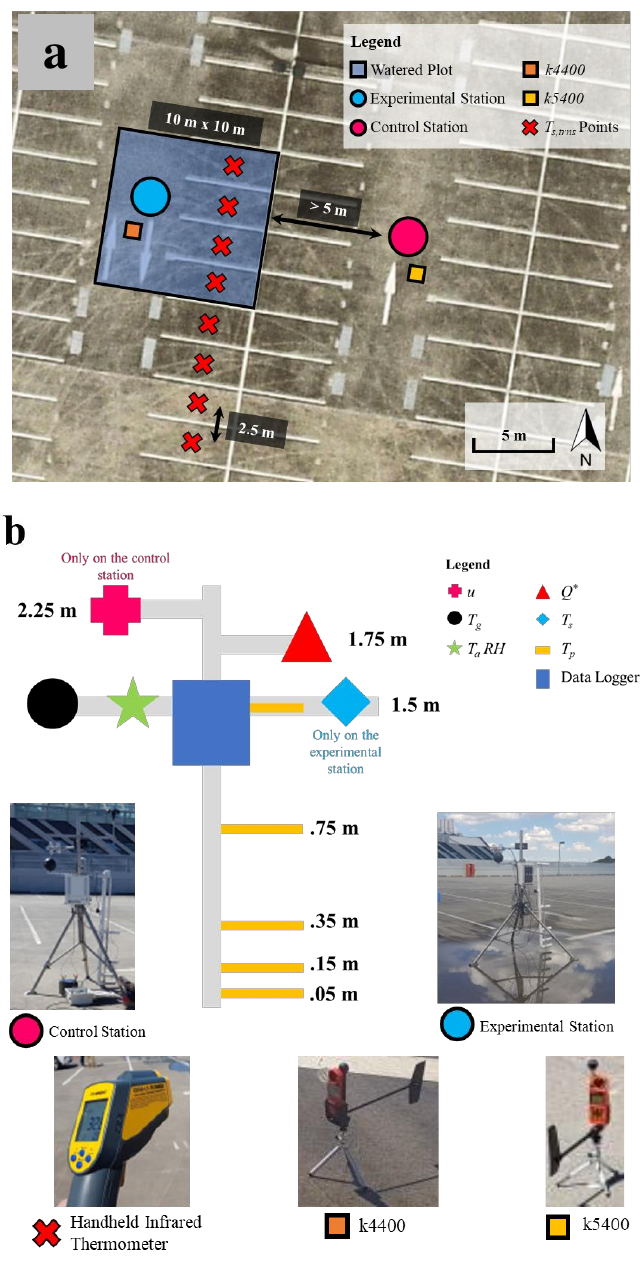
\includegraphics[trim={0 0 0 0},clip,scale=1.0]{pict001b.png}
\caption{\bf The experiment site and setup, showing (a) an aerial view of the site (adapted from \cite{Nearmap2022}); and (b) a conceptual diagram of the weather stations. The control station and kestrel (k5400) positions were not fixed, as they were moved to ensure they were upwind of the watered plot. Sensor details are given in Table \ref{table:2.1}.}
 \label{fig:2.1}
\end{figure}

\begin{table}[!ht]\caption{The sensors used in the pavement watering experiments. The symbols correspond to those used in Figure \ref{fig:2.1}.}
    \centering
   \footnotesize 
    \begin{tabular}{|p{0.90cm}|p{2.0cm}|p{2.0cm}|p{3.5cm}|p{2.5cm}|p{1.0cm}|p{1.0cm}|}
    \hline
        Symbol & Sensor & Model & Variable(s) & Accuracy & Amount & Height(s) \\ \hline
        
\includegraphics[trim={0 0 0 0},clip,scale=0.5]{Picture1.png}& Anemometer & NRG 40C & Wind speed (\gls{u}) & Within 0.1$ms^{-1}$ (between 5 to 25$ms^{-1}$) & 1 (control) & 2.25m  \\ \hline
        
\includegraphics[trim={0 0 0 0},clip,scale=0.5]{Picture2.png}& Thermistor within black sphere & Campbell Scientific BlackGlobe & Globe temperature (\gls{tg}) & $\pm$0.3$^{\circ}$C (between -3$^{\circ}$C to 90$^{\circ}$C) & 2 & 1.5m  \\ \hline               

\includegraphics[trim={0 0 0 0},clip,scale=0.5]{Picture3.png} &Temperature and Relative Humidity Probe &Campbell Scientific HMP45C&Air temperature (\gls{ta})&$\pm$0.2$^{\circ}$C at 20$^{\circ}$C, $\pm$0.3$^{\circ}$C at 40$^{\circ}$C &2&1.5m \\ 
  &&&Relative humidity (\gls{rh})&$\pm$2\% (0\% to 90\%)&& \\ \hline

\includegraphics[trim={0 0 0 0},clip,scale=0.5]{Picture4.png}&Net Radiometer (with attached thermocouple) &Campbell Scientific CNR1 (Type E thermocouple)&Incoming solar (\gls{Kdown}), outgoing solar (\gls{Kup})
Incoming far infrared (\gls{Ldown}),
Outgoing far infrared (\gls{Lup})
Net radiation (\gls{Qstar})&$\pm$10\% (for the daily totals of each component)&2&1.75m \\ \hline 

\includegraphics[trim={0 0 0 0},clip,scale=0.5]{Picture5.png}&Infrared Radiometer&Campbell Scientific SI-111&Surface temperature (\gls{ts})&$\pm$0.2$^{\circ}$C (between -10$^{\circ}$C to 90$^{\circ}$C)&1 (experimental)&1.5m \\ \hline   

\includegraphics[trim={0 0 0 0},clip,scale=0.5]{Picture6.png}&Thermocouple&Type E&Air temperature profile (\gls{tp})&Greater of $\pm$1.7$^{\circ}$C or $\pm$0.5\%&10&1.5m, 0.75m, 0.35m, 0.15m, 0.05m \\ \hline     

\includegraphics[trim={0 0 0 0},clip,scale=0.5]{Picture7.png}&Handheld Weather Meter&Kestrel 4400 (k4400)&Air temperature (\gls{Kt}), Relative humidity (\gls{Krh}), Wind speed (\gls{Ku})&±0.5$^{\circ}$C, $\pm$3\%, $\pm$0.1 ms$^{-1}$ or 3\% of reading&1 (experimental)&0.3m \\ \hline

\includegraphics[trim={0 0 0 0},clip,scale=0.5]{Picture8.png}&Handheld Weather Meter&Kestrel 5400 (k5400)&Air temperature (\gls{Kt}), Relative humidity (\gls{Krh}), Wind speed (\gls{Ku})&$\pm$0.5$^{\circ}$C, $\pm$2\%, $\pm$0.1 ms$^{-1}$ or 3\%&1 (control)&0.3m \\ \hline 

\includegraphics[trim={0 0 0 0},clip,scale=0.5]{Picture9.png}&Handheld Infrared Thermometer&Omega O5425-LS&Surface temperature (\gls{tstrns})&$\pm$1$^{\circ}$C at 20$^{\circ}$C, $\pm$0.3$^{\circ}$C at 40$^{\circ}$C&1&-1m \\ \hline           
\end{tabular}\label{table:2.1}
\end{table}



Experiments were conducted on four days in February 2022 (the 7th, 8th, 12th, and 13th). On each of these days, the maximum temperature exceeded 28$^{\circ}$C and there was no precipitation (see \ref{sec:appendix7.2} for the general daily conditions). Data from the first day of experiments (the 7th) was excluded from results due to initial setup errors. Similar to \cite{Middel2021}, watering was done at midday (M), in the afternoon (A), and in the evening (E) in an attempt to capture the effects of pavement watering during peak incoming solar radiation (\gls{Kdown}), peak air temperature (\gls{ta} and \gls{tp}), and after sunset (negative net energy, \gls{Qstar}) respectively.

Initially, a volume of 100L was used before being reduced to 60L to avoid excess runoff. On the 13th , an additional 20L of water was applied every 15 minutes for two experiments to test the impacts of more frequent watering. See Table \ref{table:2.2} for a summary of experiments, where each experiment is named after the experiment date and the time of watering.

\begin{table}[!ht]\caption{Experiment details, excluding experiments conducted on the 7th due to setup errors.}
    \centering
    \begin{tabular}{|p{2.0cm}|p{3cm}|p{2.0cm}|p{2.0cm}|p{5cm}|}
    \hline
        Date & Key & Watering Time/s & Watering Amount/s & Notes \\ \hline
        \multirow{3}{2pt}{08.02.2022} & 08M & 11:40 & 100L & \multirow{3}{*}{\parbox{4cm}{Significant water leakage, reached carpark edge}} \\
         ~ & 08A & 14:55 & 100L & ~ \\ 
         ~ & 08E & 19:30 & 100L & ~ \\ \hline
         \multirow{3}{2pt}{12.02.2022} & 12M & 11:58 & 60L & \multirow{3}{*}{\parbox{4cm}{Water leakage still present, but more controlled}} \\
          ~ & 12A & 15:32 & 60L & ~ \\ 
          ~ & 12E & 19:30 & 60L & ~ \\ \hline
        \multirow{3}{2pt}{13.02.2022} & 13M & 12:00, 12:15, 12:30, 12:45 & 60L (20L $\times$ 3) & \multirow{3}{*}{\parbox{4cm}{Water leakage same the 12th, errors in $T_{p,1.5}$, $T_{p,0.15}$, and \gls{tg} that were fixed before 13E}} \\
         ~ & 13A & 15:58, 16:15, 16:30, 16:45 & 60L (20L $\times$ 3) & ~ \\ 
         ~ & 13E & 19:26 & 60L & ~ \\ \hline
    \end{tabular}\label{table:2.2}
\end{table}

\subsection{Data Processing}\label{sec:methods2.2}
\subsubsection{Sensor Validation}\label{sec:methods2.2.1}

A validation period was conducted to ensure that control and experimental sensors were
comparable. To do this, sensors were placed side by side in a lab after the pavement
watering experiments. Ideally, sensors should be calibrated before experiments \citep{Phillips2001}, but this was not possible due to preparation being severely impacted by COVID-19 and timing constraints. The Type E thermocouples
were not included in the validation period, as they frequently required replacement
throughout the experiments. However, as all thermocouples were made from the same
cable roll using the same procedure, this was initially considered acceptable.

The validation period showed that the \gls{ta}, \gls{rh}, \gls{Krh}, \gls{Ldown}, and \gls{Lup} sensors were not directly comparable. The \gls{ta} readings showed several unnatural readings during the experiment and validation period (e.g., -40$^{\circ}$C), and thus was discarded in favour of $T_{p,1.5}$, which also captured air temperature at 1.5m. For \gls{rh} and \gls{Krh}, the mean difference between the sensors was calculated and applied to the data. 

The internal net radiometer \gls{Ldown} and \gls{Lup} calculations consider the measured sensor temperature (\gls{tcnr1}). It was found that the difference in \gls{tcnr1} was causing the inconsistencies in \gls{Ldown} and \gls{Lup} readings. Subsequent tests showed that it was likely that the experimental \gls{tcnr1} sensor was inaccurate. Therefore, it was assumed that the actual \gls{tcnr1} did not vary between the control and experimental sensors, thus \gls{Ldown} and \gls{Lup} was corrected by recalculating them using the control sensor temperature. More details on the validation period and corrections can be found in \ref{sec:appendix7.3}.

\subsubsection{Derived Variables}\label{sec:methods2.2.2}

Additional variables were derived based on the observed data acquired from the
experiments, namely wind speed at 10m (\gls{u10}), surface temperature (\gls{tsdrvd}), vapour-pressure deficit (\gls{vpd}), mean radiant temperature (\gls{Tmrt}), Universal Thermal Climate Index (\gls{utci}, a widely used measure of heat stress in outdoor spaces \citep{Zare2018a}), and components of the surface energy balance (\gls{seb}).

The wind profile power law \citep{Manwell2010,Banuelos-Ruedas2010} was
utilised with \gls{u} and \gls{Ku}  to derive \gls{u10} (\ref{sec:appendix7.4.1}). The relationship between \gls{ts} and \gls{Lup} \citep{Oke2017} was used to calculate \gls{tsdrvd} (\ref{sec:appendix7.4.2}). \gls{vpd} was calculated using $T_{p,1.5}$ and \gls{rh} \citep{Allen1998,McMahon2013} (\ref{sec:appendix7.4.3}). The python library pythermalcomfort \citep{Tartarini2020} was used to calculate \gls{Tmrt} and \gls{utci}, the former using \gls{tg}, $T_{p,1.5}$ , and \gls{u10}, and the latter using $T_{p,1.5}$, \gls{Tmrt}, \gls{rh}, and \gls{u10} (\ref{sec:appendix7.4.4}).

The \gls{seb} was also calculated. It can be simplified as:

\begin{equation}
Q^{*} = Q_{H} + Q_{E} + \Delta Q_{S}
\label{eq:2.1} 
\end{equation}

where \gls{Qstar} is the net all radiation ($Wm^{-2}$) (i.e., (\gls{Kdown} - \gls{Kup}) + (\gls{Ldown} - \gls{Lup})), \gls{Qh} is the sensible heat flux ($Wm^{-2}$), \gls{Qe} is the latent heat flux ($Wm^{-2}$), and \gls{deltaqs} is the change in heat storage ($Wm^{-2}$) (Oke et al. 2017). The mean \gls{Qe} from the start of watering to the approximate drying time was estimated based on the amount of water and the approximate evaporation time. \gls{Qh} was calculated based on \gls{tsdrvd}, \gls{tp}$_{,0.05}$, and \gls{u10} \citep{Liu2007}, as well as roughness lengths from \cite{Kanda2007}, while \gls{Qstar} was directly measured. The mean \gls{Qh} and \gls{Qstar} from the wet period was calculated, allowing the mean \gls{deltaqs} to be estimated as the energy balance residual \citep{Oke2017}. These mean values were also used to calculate the Bowen ratio (\gls{bowen} = \gls{Qh} / \gls{Qe}) alongside the ratio of \gls{Qh} to \gls{Qstar} (\gls{Qh} / \gls{Qstar}) \citep{Oke2017}. See \ref{sec:appendix7.4.5} for details.


\subsubsection{Statistical Analysis}\label{sec:methods2.2.3}

The difference between the control and experimental sites was calculated (\gls{delta} =
experimental - control, thus \gls{delta} $<$ 0 indicates cooling). Preliminary analysis showed that even after applying corrections to account for incompatible sensors, differences between the control and experimental variables still existed before watering took place. These differences varied between the experiments and observational variables, and are explored with more detail in the results. As the expected impact of watering is small, these relatively small pre-existing differences can exaggerate or diminish the actual impact of pavement watering, depending on the initial bias.

Thus, for the purposes of this study, impacts were assessed by evaluating changes relative to the initial difference. Specifically, the average difference between the control and experiment before watering (\gls{deltadry}), taken as a maximum of 30 minutes before watering, was compared to the average difference during the wet period (\gls{deltawet}), which was defined as when watering was finished to when it was dry under the experimental station (for experiments with repeated applications of water, the end of the initial watering was used). In other words, the observed cooling impact of pavement watering (\gls{pwimpact}) in a particular experiment was defined as:

\begin{equation}
PW_{impact} = \bar{\Delta}_{wet} - \bar{\Delta}_{dry}
\label{eq:2.2} 
\end{equation}

An independent t-test was also conducted to verify if \gls{deltawet} was significantly lower (or significantly greater for \gls{rh}) than \gls{deltadry}. The effect of prevailing conditions on the effectiveness of pavement watering was also explored. To do this, the \gls{pwimpact}, as well as \gls{Qe}, were compared to mean of prevailing conditions during the wet period via linear regression. The statistical significance of a non-zero slope was calculated. For the surface temperature transects (\gls{tstrns}), the difference between the mean of the watered points and non-watered points was calculated (i.e., \gls{deltatstrns} = $\overline{T}_{s,trns,wet} - \overline{T}_{s,trns,dry}$), and a t-test was again used to verify if the watered points were significantly less than non-watered plots. A \gls{p}-value of less than 0.05 was used to validate significance in all cases.

\section{Results}\label{sec:discussion3}
\subsection{Air Temperature}\label{sec:discussion3.1}

An air temperature profile, comprised of temperature observations at five heights (0.05m to 1.5m), was measured at the experimental and control site (\gls{tp}, see Figure \ref{fig:2.1}b). The difference was calculated between the temperatures of the same height ($\Delta$\gls{tp}). Air temperature at a specific height is referred to as $T_{p,height}$ and likewise differences at a specific height is referred to as $\Delta$$T_{p,height}$.

As detailed in Section \ref{sec:methods2}, there were differences between the experimental and control \gls{tp} before watering was conducted (i.e., $\Delta$\gls{tp} $\neq$ 0 before watering). The $\Delta$\gls{tp} before watering was found to be variable between the experiments and the different \gls{tp} heights. In the evening experiments, $\Delta$\gls{tp} was predominantly less than zero, indicating that the experimental site already was cooler than the control site before watering, while midday and afternoon experiments had a mixture of both less and greater than zero (Figure \ref{fig:7.9}). Given the apparently random nature of these pre-existing differences at different heights, it is likely they are not reflective of the actual temperature differences between the sites.

The relationship between pre-existing differences and the absolute control temperature (\gls{tpcon}) as well as wind speed (\gls{u10}) was investigated. The $\Delta$\gls{tp} before watering was found to have a statistically significant relationship with \gls{tpcon} for each individual experiment and height, apart from experiment 13E at 1.5m (Figure \ref{fig:7.10}). A relationship with \gls{u10} was also found, however it was not as consistently statistically significant (Figure \ref{fig:7.12}). There were no significant relationships when considering all the experimental data together, likely as \gls{tp} sensors frequently malfunctioned and were replaced, and as the control station was moved to ensure it remained upwind of the watered plot. Thus, $\Delta$\gls{tp} was detrended based on the linear relationship derived for each individual experiment and height in an attempt to remove factors that caused the observed differences between sites that were unrelated to pavement watering. However, it was found that results were biased by the changes in \gls{tpcon} and \gls{u10} values throughout the experiment.

Figure \ref{fig:3.1} highlights these issues with an example of observed temperature differences for experiment 12M at 0.15m. The $\Delta$$T_{p,0.15}$ was already less than zero before watering, and thus the cooling of pavement watering would be exaggerated if simply taken as the difference between the experimental and control site when the surface is wet (Figure \ref{fig:3.1}c). Despite this, there was still a clear negative shift in $\Delta$$T_{p,0.15}$ when the surface was wet, indicating that pavement watering may have a cooling effect. Thus, it was possible to derive the impact of pavement watering by simply shifting the observed differences based on the mean of the before watering period, however this assumes that the pre-existing differences were constant (Figure \ref{fig:3.1}c).

\begin{figure}
\centering
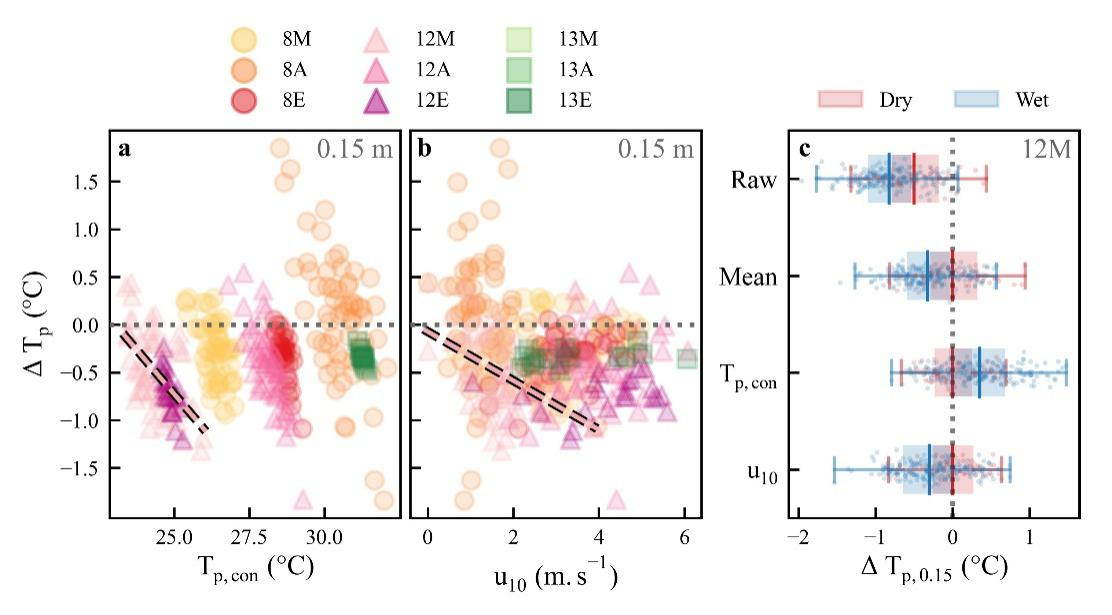
\includegraphics[trim={0 0 0 0},clip,scale=1.2]{pict011.jpg}
\caption{\bf A scatter plot of before watering $\Delta$\gls{tp} vs (a) \gls{tpcon} and (b) \gls{u10} for each experiment at 0.15m, with the pink line outlined in black showing the linear relationship for experiment 12M. (c) Boxplots of $\Delta$\gls{tp} for dry (before watering) and wet periods of experiment 12M at 0.15m with different corrections applied (raw: no correction, mean: shifted based on dry mean, \gls{tpcon}: detrended based on linear relationship in (a), \gls{u10}: detrended based on linear relationship in (b).}
 \label{fig:3.1}
\end{figure}

The linear relationship between the pre-existing $\Delta$$T_{p,0.15}$ and \gls{tpcon} at the same height is shown in Figure \ref{fig:3.1}a (p $<$ 0.01), and the $\Delta$$T_{p,0.15}$ detrended with this relationship is shown in Figure \ref{fig:3.1}c. This corrected $\Delta$$T_{p,0.15}$ shows a positive shift in differences after watering (i.e., the experimental site becoming warmer than the control). However, this was likely due to temperatures increasing throughout the midday experiment, beyond the values used to calculate the applied linear model. As higher temperature was related to a more negative $\Delta$$T_{p,0.15}$ , the corrected $\Delta$$T_{p,0.15}$ reflected the change in \gls{tpcon} relative to before watering rather than isolating the impacts of pavement watering. This was also seen as the detrended $\Delta$\gls{tp} based on \gls{tpcon} generally showed no cooling from pavement watering for midday experiments where temperatures increased through the experiment, and high cooling for evening experiments where temperature progressively decreased (Figure \ref{fig:7.11}).

The same problems were seen when correcting $\Delta$\gls{tp} based on its relationship with wind speed. Figure \ref{fig:3.1}b shows the linear relationship between pre-existing $\Delta$$T_{p,0.15}$ and \gls{u10} (\gls{p} $<$ 0.01), and the corresponding corrected $\Delta$$T_{p,0.15}$ is shown in Figure \ref{fig:3.1}c. The corrected $\Delta$$T_{p,0.15}$ is somewhat similar to correcting $\Delta$$T_{p,0.15}$ based on the mean of the pre-existing differences. The shift in \gls{u10} values before and after watering was not as acute as with \gls{tpcon}, however it still likely leads to unintended side-effects, including increasing the variability of $\Delta$$T_{p,0.15}$ when it is wet.

Thus, to avoid the uncertainties associated with the extrapolation of the calculated linear models, the $\Delta$\gls{tp} relative to the mean before watering was chosen to assess the impacts of pavement watering. Figure \ref{fig:3.2} shows the raw and mean corrected $\Delta$\gls{tp} for experiment 8M. The corrected $\Delta$\gls{tp} shows that watering generally had a decreasing impact with increasing height. There also was an immediate cooling effect, especially at lower heights. After the surface dried, some temperatures differences returned to the established baseline (the mean of the before watering differences), however they also often increased, or decreased, relative to the baseline. This can be seen in both Figure \ref{fig:3.1}b as well as the other experiments (Figure \ref{fig:7.14}). It is difficult to be certain of the long-term effects given the apparent instability of the measured differences between the control and experimental site, and thus the true impact of pavement watering.

\begin{figure}
\centering
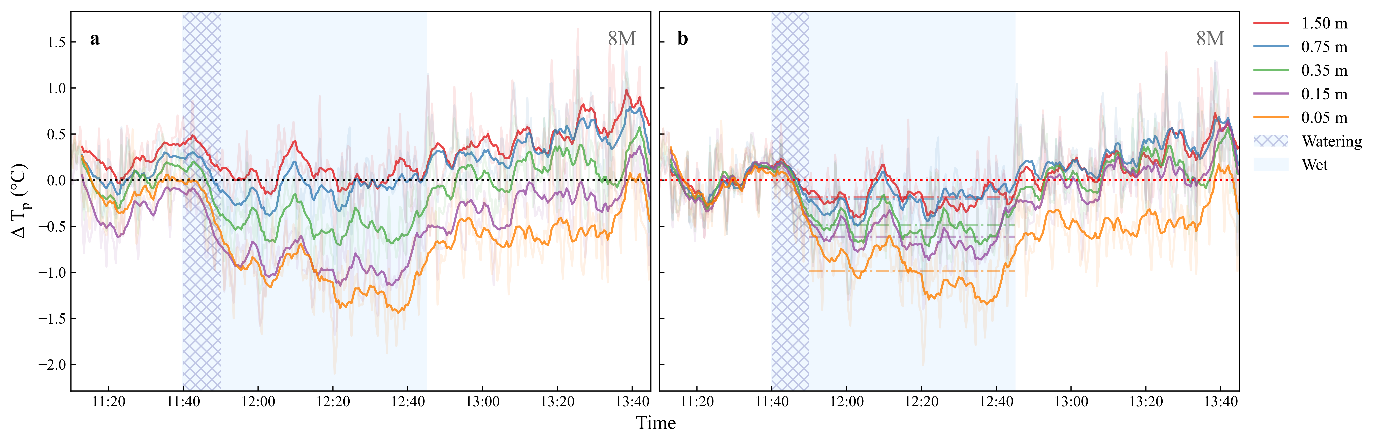
\includegraphics[trim={0 0 0 0},clip,scale=1.1]{pict013.png}
\caption{\bf \gls{tp} differences for experiment 8M (a) with no correction and (b) corrections based on the mean of before watering. The transparent lines represent the raw data, while the solid lines are the 5-minute running average. The shading indicates periods when the pavement was wet, and the hatching shows when watering was being conducted. The dashed lines on (b) represented the mean of the wet period.}
 \label{fig:3.2}
\end{figure}

To overcome these challenges and uncertainties, the cooling impact of pavement watering on air temperature was taken as the mean difference during the wet period relative to the mean difference before watering (i.e., \gls{pwimpact} for \gls{tp}, see Equation \ref{eq:2.2}). The \gls{pwimpact} for \gls{tp} varied from no observable decrease to a cooling of up to 1$^{\circ}$C, with the exception of 2.5$^{\circ}$C at 0.05m for experiment 8A (Figure \ref{fig:3.3}a). Consistent with Figure \ref{fig:3.3}b, cooling generally decreased with height (Figure \ref{fig:3.3}a). Considering all experiments, the evening experiments had the lowest air temperature cooling at 0.05m, however there was no clear decrease in cooling for evening experiments at other \gls{tp} heights. However, considering individual experiment days, the cooling was generally greatest in the afternoon and lowest in the evening, especially at lower heights.

\begin{figure}
\centering
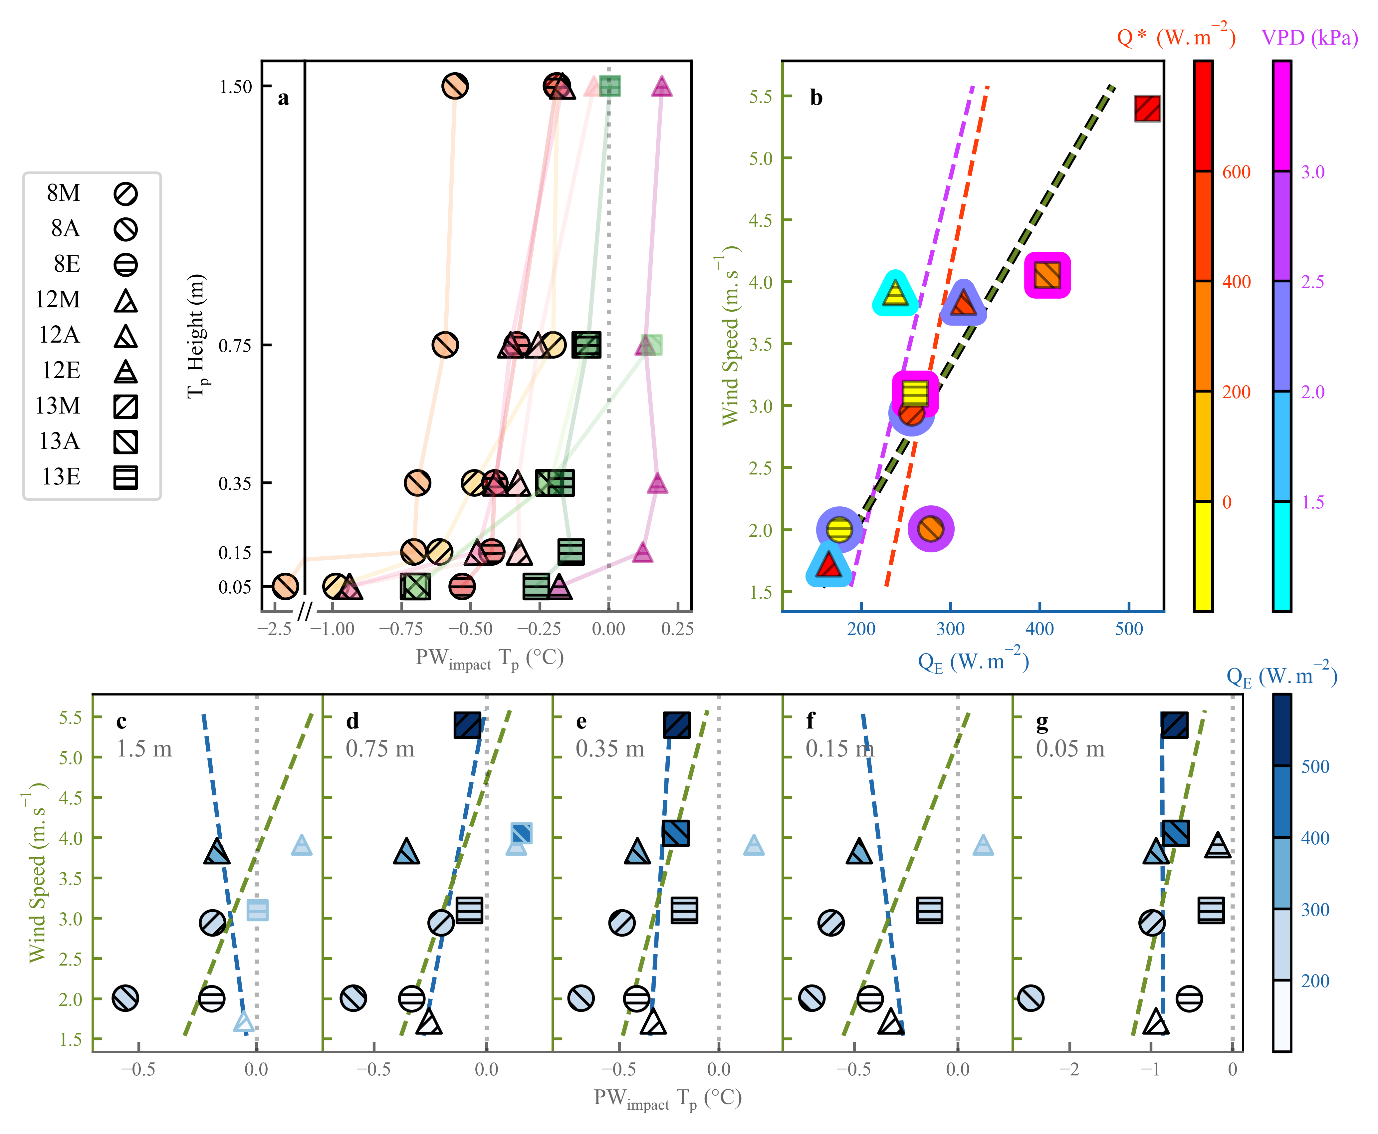
\includegraphics[trim={0 0 0 0},clip,scale=1.0]{pict014.png}
\caption{\bf (a) The \gls{pwimpact} for \gls{tp} at each \gls{tp} height, where each scatter marker colour indicates a separate experiment. Note the x-axis is discontinuous. (b) the relationship between \gls{Qe} and the mean \gls{u10} (y-axis, green dashed line), the experimental \gls{Qstar}, (red dashed line, colour of scatter marker) and the experimental \gls{vpd} (purple dashed line, border colour of scatter marker) during the wet period; (c-g) \gls{pwimpact} for \gls{tp} vs \gls{u10} y-axis, (green dashed line) and \gls{Qe} (blue dashed line, colour of scatter marker) at each \gls{tp} height. A black outline for the scatter points indicates a statistically significant change in \gls{tp} (a, c-g), while a black outline on the dashed line indicates a statistically significant linear relationship (b, c-g).}
 \label{fig:3.3}
\end{figure}

Given the spread in results, the specific conditions during individual experiments were investigated. Namely, as pavement watering utilities evaporative cooling, firstly the impact of prevailing conditions known to influence \gls{Qe} was explored (Figure \ref{fig:3.3}b). \gls{Qe} was found to be positively correlated to \gls{u10} (\gls{p} $<$ 0.01, \gls{r2} = 0.74), and also related to experimental \gls{vpd} and \gls{Qstar} (\gls{r2} = 0.31 and 0.15 respectively), although these relationships were not statistically significant (\gls{p} = 0.15 and 0.30 respectively) (Figure \ref{fig:3.3}). As expected, \gls{Qstar} was found to be highly correlated to \gls{Kdown} (\gls{r2} = 0.99), suggesting that solar radiation was a key source of energy for \gls{Qe}.

However, there was no strong correlation between air temperature cooling and \gls{Qe}. \gls{Qe} had a slight positive correlation with air temperature cooling at 0.75 m (\gls{r2} = 0.11) and 0.35 m (\gls{r2} = 0.01), a weak negative relationship at 1.5m (\gls{r2} = 0. 07) and 0.15m (\gls{r2} = 0.05), and no impact at 0.05m (\gls{r2} $<$ 0.01). Additionally, none of these relationships were statistically significant (\gls{p} $>$ 0.4) (Figure \ref{fig:3.3}c-g). The weak negative relationship at 1.5m and 0.15m was likely due to the malfunctions at those heights for experiment 13M and 13A, which had high \gls{Qe} and low cooling at other heights. Thus, high \gls{Qe} was marginally related to reduced air temperature cooling.

On the other hand, air temperature cooling was found to be related to wind speed. Lower \gls{u10} related to more cooling across all \gls{tp} heights (\gls{r2} ranged from 0.15 to 0.36), although again these relationships were statistically insignificant (\gls{p} $>$ 0.09) (Figure \ref{fig:3.3}c-g).

Air temperature was also recorded at 0.3m with the Kestrels (\gls{Kt}) (Figure \ref{fig:2.1}a). However, this was impacted by rather extreme pre-existing differences, with $\Delta$\gls{Kt} before watering found to be up to 6$^{\circ}$C. Additionally, the \gls{pwimpact} for \gls{Kt} (Equation \ref{eq:2.2}) did not align with results from the temperature profile, with a maximum cooling of 0.84$^{\circ}$C (13A) and maximum warming of 0.61$^{\circ}$C (13M) (Table \ref{table:7.4}). Although the Kestrels were tested in the validation period and appeared to be compatible (\ref{sec:appendix7.3}), the two Kestrels may have responded differently in the relatively dynamic, hot carpark environment, especially when compared to a lab environment. Thus, these results are disregarded given that two different Kestrel models were potentially inappropriate for the purposes of this experiment.

Overall, pavement watering was found to reduce air temperature, with a maximum decrease of 0.6$^{\circ}$C and 2.5$^{\circ}$C found at 1.5m and 0.05m respectively. Despite the uncertainties associated with the differences between the control and experimental observations, the derived impact of pavement watering on air temperature was within estimates from other field studies (see \ref{sec:appendix7.1}, Table \ref{table:7.2}), and indeed align with expectations, for example decreased cooling with height. The impact of pavement watering was also found to be dependent on prevailing conditions, especially wind speed, but was not found to be strongly correlated with \gls{Qe}.

\subsection{Thermal Comfort}\label{sec:discussion3.2}

The thermal comfort benefits of pavement watering was assessed using \gls{utci}. This, as well as \gls{Tmrt}, was calculated with observational $T_{p,1.5}$, \gls{rh}, \gls{tg}, and \gls{u10}. As detailed above, the air temperature at 1.5m was significantly different between the control and experimental station before watering took place. \gls{rh} and \gls{tg} also had pre-existing differences, and like \gls{tp}, this varied with the experiments. Nevertheless, these observations were used to calculate \gls{Tmrt} and \gls{utci}, and thus these variables also inherited pre-existing differences. Thus, as with air temperature, the \gls{pwimpact} (Equation \ref{eq:2.2}) was used to derive the impact of pavement watering.

The \gls{pwimpact} for \gls{utci} and all its components, save wind speed, which was considered the same across the entire carpark, is shown in Figure \ref{fig:3.4}. \gls{utci} was found to be reduced by 0.2$^{\circ}$C to 2.0$^{\circ}$C by pavement watering, despite watering generally increasing \gls{rh} (-0.02\% to 1.19\%). It should be noted that spikes in \gls{rh} were seen at the experimental site after watering, which was not captured by the \gls{pwimpact}. 

\gls{Tmrt} was found to drive \gls{utci} changes, except in experiment 12M and 12E where there was little observable air temperature cooling. \gls{Tmrt} in turn was driven by reductions in \gls{tg}, except for experiment 12E. As with air temperature, for individual experiment days, the \gls{utci} reduction is greatest in the afternoon and lowest in the evening. Reduction in \gls{tg} due to watering is weakest during the evening, which also leads to a lower \gls{utci} reduction in the evening. In summary, pavement watering was found to improve thermal comfort. Despite observed increases in \gls{rh}, reductions in air temperature and globe temperature resulted in reducing \gls{utci} by a maximum of 2.0$^{\circ}$C.

\begin{figure}
\centering
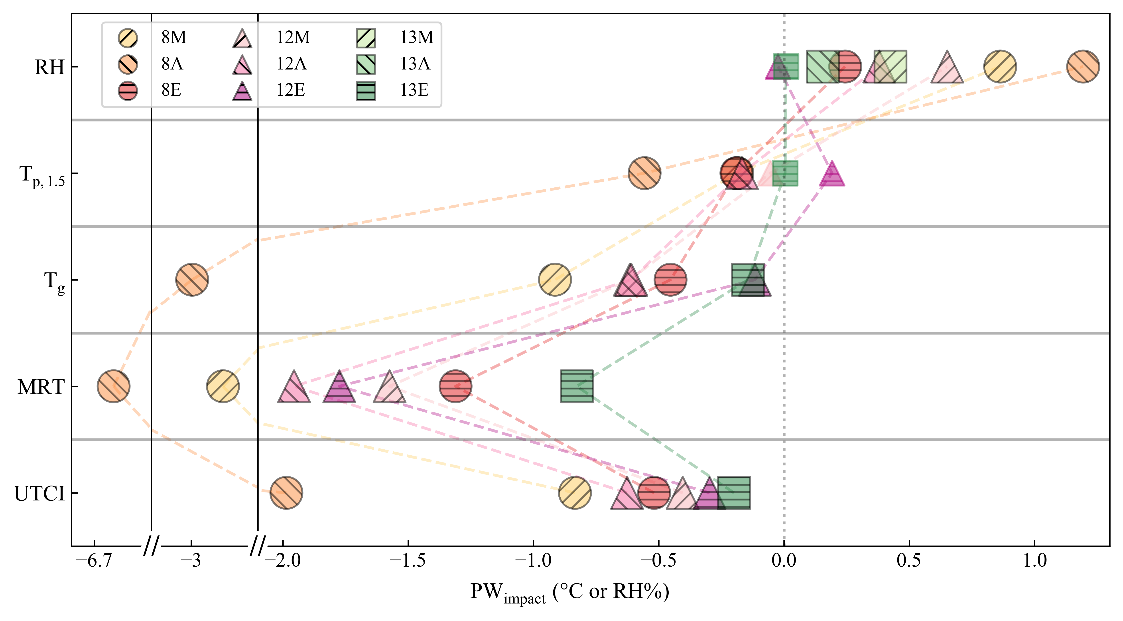
\includegraphics[trim={0 0 0 0},clip,scale=1.2]{pict015.png}
\caption{\bf The \gls{pwimpact} for \gls{utci} and its variables (\gls{rh}, $T_{p,1.5}$ , \gls{tg}, and \gls{Tmrt}) for each experiment. The black outline indicates a statistically significant impact from watering for a particular variable (\gls{p} $<$ 0.05). Note the x-axis is discontinuous.}
 \label{fig:3.4}
\end{figure}


\subsection{Surface Temperature}\label{sec:discussion3.3}

The surface temperature was measured via transects (\gls{tstrns}) with one handheld infrared thermometer, with 4 points outside the designated watered plot and 4 within (Figure \ref{fig:2.1}a). A single transect was done before watering, allowing for the investigation of actual differences within the sites before watering takes place. Additionally, surface temperature was derived (\gls{tsdrvd}) for the control and experimental station using \gls{Lup} and verified with observations from the one available continuous surface temperature sensor on the experimental station. \gls{deltatstrns} refers to the difference between the mean surface temperature of the watered points and the mean of the non-watered points, while $\Delta$\gls{tsdrvd} refers to the difference between the experimental and control derived surface temperature.

Figure \ref{fig:3.5} shows the surface temperature transects for experiment 13E, alongside the \gls{deltatstrns} for all experiments. Both these figures show that watering resulted in a clear reduction in surface temperature, and this cooling remained significant even after the surface visibly dried. The heterogeneity of the carpark surface is also apparent in Figure \ref{fig:3.5}a. The greatest difference within the control points for the same transect was 3.8$^{\circ}$C (12A), and 8.4$^{\circ}$C (8A) for experimental points (Figure \ref{fig:7.15}), the latter potentially due to the different drying rates across the watered plot.

\begin{figure}
\centering
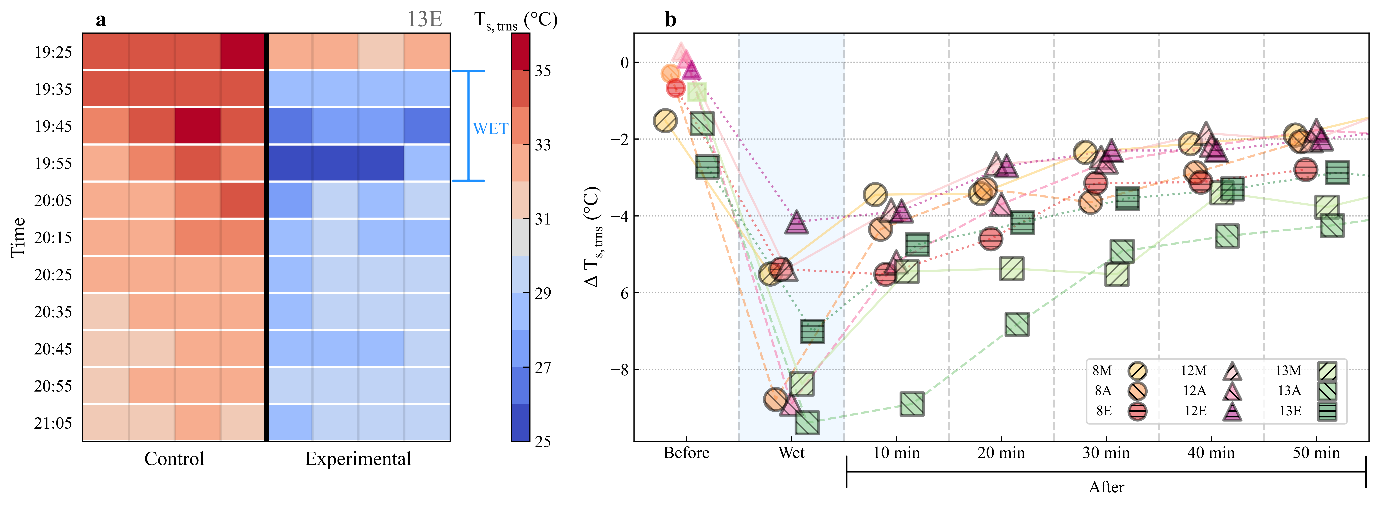
\includegraphics[trim={0 0 0 0},clip,scale=1.05]{pict016.png}
\caption{\bf (a) The \gls{tstrns} of experiment 13E showing the evolution from before, during, and after the wet period (rows) for control and experimental points along the transect (columns); (b) the \gls{deltatstrns} of all experiments, where the wet refers to the mean \gls{deltatstrns} of the wet period. The black outline indicates that the experimental points are statistically significantly lower than the control points (\gls{p} $<$ 0.05).}
 \label{fig:3.5}
\end{figure}

It is also evident that \gls{deltatstrns} was usually less than zero before watering, and this difference was statistically significant for three experiments (Figure \ref{fig:3.5}b). With the exception of experiment 8M, the magnitude of these before watering differences increased throughout the day (e.g., 13M $<$ 13A $<$ 13E) (Figure \ref{fig:3.5}b). This suggests that the effect of watering lasted beyond a given experiment, and has a long-lasting cooling impact on surface temperature. This is also shown in the derived surface temperature, where there was little differences between control and experimental sites before the midday experiment (-0.2$^{\circ}$C to -0.5$^{\circ}$C), followed by a significantly cooler experimental surface temperatures before the afternoon (-1.7$^{\circ}$C to -2.2$^{\circ}$C) and evening (-1.8$^{\circ}$C to -3.4$^{\circ}$C) experiments (Figure \ref{fig:7.17} and Table \ref{table:7.5}).

In an attempt to isolate the experiments, the \gls{deltatstrns} was also calculated relative to the transect done before watering. A mean decrease of 4.0$^{\circ}$C to 9.0$^{\circ}$C was observed during the wet period for the isolated experiments (Figure \ref{fig:7.16}). The raw mean decrease in surface temperature can be taken as the cumulative impact of pavement watering, and this was slightly higher (4.2$^{\circ}$C to 9.3$^{\circ}$C) (Figure \ref{fig:3.5}b).

As derived surface temperature was observed regularly, the impact of pavement watering for each individual experiment can be derived with \gls{pwimpact} (Equation \ref{eq:2.2}). Pavement watering decreased \gls{tsdrvd} by 2.1$^{\circ}$C to 6.8$^{\circ}$C, however it should be noted that experimental \gls{tsdrvd} does not completely capture the minimum surface temperature observations (as measured by the observational \gls{ts} sensor), and thus these results are likely underestimated (Figure \ref{fig:7.17} and Table \ref{table:7.5}). Similar to the \gls{deltatstrns}, the cumulative impact of watering on surface temperature can be taken as the mean during the wet period without any corrections. The cumulative decrease seen in \gls{tsdrvd} was 3.7$^{\circ}$C to 7.3$^{\circ}$C (Figure \ref{fig:7.17} and Table \ref{table:7.5}).

In all measures of surface temperature, there was generally lower individual reductions in the evening experiments, although this was partially compensated with the cumulative cooling from previous experiments. The highest individual and cumulative cooling was seen in the afternoon, likely as the experimental surface reached its peak temperature in the period before the afternoon experiment (Figure \ref{fig:7.17} and Table \ref{table:7.5}).

In general, the surface temperature cooled by up to 9.0$^{\circ}$C due to pavement watering. The watered surface remained noticeably cooler than the non-watered surface even after the water visibly dried, and likely led to cumulative cooling for each subsequent experiment within the individual experiment days. Thus, pavement watering was shown to significantly reduce surface temperature when wet and have a prolonged cooling effect even after the surface dried.

\subsection{Surface Energy Balance}\label{sec:discussion3.4}

The surface energy balance (\gls{seb}) was simplified to net radiation (\gls{Qstar}), latent heat flux (\gls{Qe}), sensible heat flux (\gls{Qh}), and change in heat storage (\gls{deltaqs}). \gls{Qstar} was directly observed, while \gls{Qe} and \gls{Qh} where calculated, the latter based largely on the derived surface temperature (\gls{tsdrvd}) at air temperature at 0.05m ($T_{p,0.05}$). Finally, \gls{deltaqs} was derived as the \gls{seb} residual. Figure \ref{fig:3.6}a shows the mean \gls{seb} during the wet period at the control and experimental site for each experiment. There is a marked impact of watering, namely the presence of \gls{Qe}, higher \gls{Qstar}, and lower \gls{Qh} and \gls{deltaqs}.

\begin{figure}
\centering
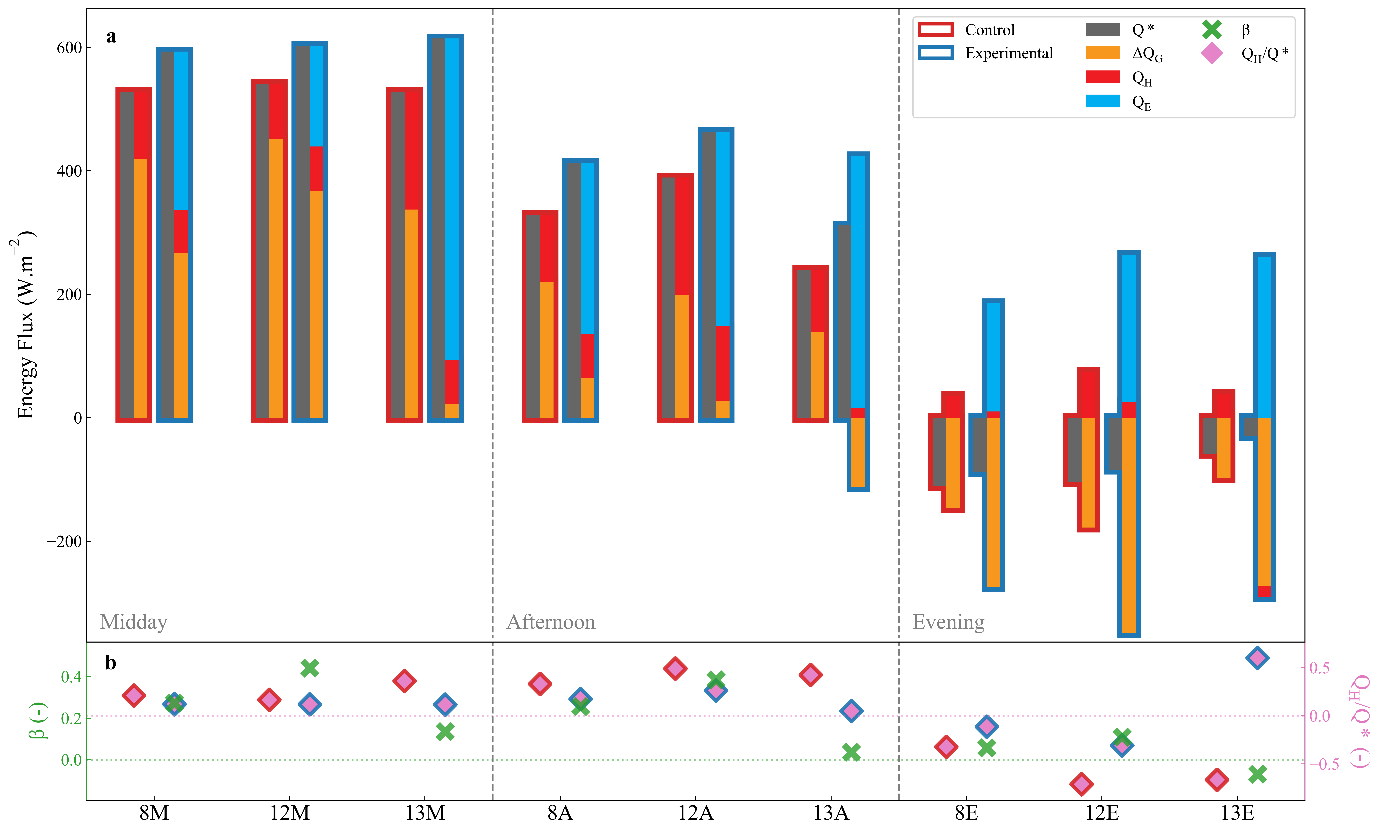
\includegraphics[trim={0 0 0 0},clip,scale=1.0]{pict017.png}
\caption{\bf (a) The mean \gls{seb} of each experiment's control and experimental site during the wet period; (b) the \gls{bowen} alongside the \gls{Qh} and \gls{Qstar} ratio for each experiment.}
 \label{fig:3.6}
\end{figure}

It was found that surface albedo and temperature decreased due to watering, leading to decreased \gls{Kup} and \gls{Lup}, and thus higher \gls{Qstar}. \gls{Qe} more than compensates for this increase in \gls{Qstar}, as a large portion of \gls{Qstar} appears to be forcing \gls{Qe} for midday and afternoon experiments, while energy is predominantly provided by \gls{deltaqs} in the evening. \gls{deltaqs} was also notably negative for experiment 13A, and \gls{Qh} was negative for 13E, suggesting that they also contributed to \gls{Qe}.

Figure \ref{fig:3.6}b shows the Bowen ratio (\gls{bowen}) alongside the \gls{Qh} to \gls{Qstar} ratio (\gls{Qh}/\gls{Qstar}) for each experiment. The \gls{bowen} ranges from 0.04 to 0.44 during the day, and from -0.07 to 0.11 in the evening. A daytime \gls{bowen} of 0.1 to 0.3 is typical of a tropical wet forest, while a \gls{bowen} of 3 to 8 is associated with urban areas with $<$ 20\% greenspace \citep{Oke2017}. Thus, it is evident that the addition of water allows otherwise the dry carpark, characteristic of an urban area, to imitate highly evaporative environments.

The difference between the experimental and control \gls{Qh}/\gls{Qstar} (i.e., the $\Delta$\gls{Qh}/\gls{Qstar}) ranges from -0.05 to -0.37 in the midday and afternoon experiments (Figure \ref{fig:3.6}b), indicating that less \gls{Qstar} was partitioned into \gls{Qh} due to watering despite increased \gls{Qstar}. For the evening experiments, $\Delta$\gls{Qh}/\gls{Qstar} ranged from 0.21 to 1.27 (Figure \ref{fig:3.6}b). This indicates that the control site had a lower \gls{Qh}/\gls{Qstar}, which is expected as \gls{Qstar} is negative, and thus still relates to a decreased \gls{Qh} at the watered site.

It should be acknowledged that existing differences before each experiments impacted the \gls{seb} and \gls{Qh}/\gls{Qstar}, as \gls{tsdrvd} and $T_{p,0.05}$ both had differences between the control and experimental site before watering, as discussed in previous sections. Analysis of the \gls{seb} in the period before watering reflected these pre-existing differences between the sites, especially for afternoon and evening experiments (Figure \ref{fig:7.18}). Thus, the actual impact of watering on $\Delta$\gls{Qh}/\gls{Qstar} can be deduced from the relative change from the $\Delta$\gls{Qh}/\gls{Qstar} before watering. This difference ranged from -0.04 to -0.24 in the midday and afternoon, and from -0.03 to 1.17 in the evening (Figure \ref{fig:7.19}). Thus, watering still resulted in a lower proportion of \gls{Qh}, except for experiment 8E, where there was little change relative to before watering took place.

However, these pre-existing differences in the \gls{seb} were largely related to the prolonged impact of watering on surface temperature (i.e., differences between the experimental and control \gls{tsdrvd} rather than $T_{p,0.05}$). This can be seen as the wet period $\Delta$\gls{Qh}/\gls{Qstar} at midday matches fairly well with the before watering $\Delta$\gls{Qh}/\gls{Qstar} in the afternoon for all experiment days (e.g., 13M $\Delta$\gls{Qh}/\gls{Qstar} when wet was close to 13A $\Delta$\gls{Qh}/\gls{Qstar} before watering), highlighting the effect of prolonged cooling of the surface temperature on the \gls{seb} (Figure \ref{fig:7.19}). Thus, as with surface temperature, the $\Delta$\gls{Qh}/\gls{Qstar} during the wet period can be taken as the cumulative impact of pavement watering (Figure \ref{fig:3.6}b), while the $\Delta$\gls{Qh}/\gls{Qstar} relative to before watering can be assumed to be the individual experiment impact.

Overall, pavement watering had a considerable impact on the \gls{seb} of the carpark. The expected characteristics of a carpark (high \gls{Qh} and \gls{deltaqs}) were seen at the control site, while the \gls{seb} for the watered section was dominated by \gls{Qe}, which is more typical of moist environments. The changes in the \gls{seb} are the driving force behind the observed cooling provided by pavement watering.

\section{Discussion}\label{sec:discussion}
 
As noted above, a key confounding factor of this study stems from the existing differences in the experimental and control observations before watering took place. Given the apparent heterogeneity of the carpark surface (Figures \ref{fig:3.5}a and \ref{fig:7.15}), it appears that there may have been slight actual differences between the sites. Moreover, experiments were not as independent as initially assumed, as both the surface temperature transects and the derived surface temperature showed a prolonged cooling due to pavement watering after the surface visibly dried (Figures \ref{fig:3.5} and Figure \ref{fig:7.17} and Table \ref{table:7.5}). However, pre-existing differences for other observations were less stable, for example the differences between the control and experimental air temperature profile changed between experiments and heights (Figure \ref{fig:7.9}).

These differences between the control and experimental air temperature observations were negatively correlated to the absolute control observations at an individual experiment level (Figure \ref{fig:7.10}), suggesting that the temperature sensors had different sensitivities. Wind speed may have also impacted the control and experimental observations in some experiments (Figure \ref{fig:7.12}), indicating that potentially the temperature sensors were not secured properly. However, attempts to isolate and remove these factors that contributed to these differences resulted in the corrected data reflecting changes in observed control temperature and wind speed, rather than potential impacts of watering (Figures \ref{fig:7.11} and \ref{fig:7.13}).

Therefore, the impact of pavement watering was deduced by comparing differences relative to the mean of the dry period. This is still not ideal, as it involves assuming that the `natural' difference during an experiment remains stationary. However, this was considered necessary, as using uncorrected data would result in overestimating or underestimating the impact of watering, depending on the initial bias. Indeed, given the alignment of results, for example the cooling impact decreasing with temperature height, it is considered an adequate representation of the impact of pavement watering.

Pavement watering's effectiveness at reducing air temperature was found to be dependent on wind (Figure \ref{fig:3.1}c-g), where lower wind speeds allowed cooling to accumulate and propagate upwards. This corresponds to pavement watering activation conditions in Paris, where wind speed needs to be less than 2.8$ms^{-1}$ \citep{Hendel2015a}.

As pavement watering utilises evaporative cooling, it was interesting to observe that \gls{Qe} had a weak correlation with air temperature, and higher \gls{Qe} was associated with less cooling at some heights (Figure \ref{fig:3.3}c-g). This is likely due to the competing effect of wind speed, where higher wind speeds were found to strongly enhance \gls{Qe} (Figure \ref{fig:3.3}b) while simultaneously limiting observed cooling.

The experiment with the highest air temperature and thermal comfort benefits (8A) had low wind speeds and average \gls{Qe}, while an experiment with lower wind speeds but low \gls{Qe} had insignificant cooling at 1.5m (12M) (Figures \ref{fig:3.3}c-g and \ref{fig:3.4}). This indicates the pavement watering is most effective when \gls{Qe} is high at low wind speeds, for example when \gls{vpd} is high.

There is a possibility that advection caused a downwind propagation of cooling, as observed in urban parks \citep{Motazedian2020}, however given the small plot being watered and lack of observations downwind, this would need subsequent tests to prove. In terms of watering time, evening experiments generally had the lowest observed cooling benefits, particularly for surface temperature, the air temperature closest to the ground ($T_{p,0.05}$), and \gls{tg}; and thus, \gls{Tmrt} and \gls{utci} by relation. The relatively low reductions in surface temperature arguably occurred as the carpark surface was already cooling down due to the lack of \gls{Kdown}, and likely influenced evening $T_{p,0.05}$ and \gls{tg}. Indeed, \cite{Takebayashi2021} found that the cooling effect of pavement watering on surface temperature was generally greater the hotter the surface temperature was, which was also reflected in this study. However, there does not appear to be a clear relationship between surface temperature and air temperature other than at 0.05m in the evening, potentially due to the stronger heat turbulence during the day and the evident influence of horizontal advection.

Despite the lower cooling benefits, pavement watering may provide key benefits in the evening. Namely, there was a negative \gls{Qh} in experiment 13E, while all other evening experiments had a positive \gls{Qh}. This likely occurred due to the prolonged cooling impact pavement watering had on surface temperature, which meant that before watering for experiment 13E, \gls{Qh} was already lower at the experimental site compared to the control. Additionally, the previous experiments of the day, 13M and 13A, had small and negative \gls{deltaqs} respectively, indicating that the accumulation of heat storage in the ground that is typical of urban surfaces \citep{Oke1982,Anandakumar1999} was severely limited by pavement watering. This in turn was likely due to the fact that both experiments were characterised by high \gls{Qe}, due to both ideal evaporation conditions (high wind speed and \gls{vpd}) and the extra water that was applied for these experiments. Thus, the previous watering throughout the day may have allowed the reversal of \gls{Qh} when watering was applied in the evening. This implies that frequent watering in the right conditions may allow urban areas to cool more effectively at night, and thus mitigate the negative health impacts of high night-time temperatures characteristic of urban areas \citep{Clarke1972,Coutts2010}.

However, it should be noted that numerous assumptions were made to calculate the \gls{seb}. Notably, \gls{deltaqs} was calculated indirectly and any advection of energy was ignored. Despite this, the \cite{Cohard2018} study on the energy budget of a carpark under simulated rainfall events, with appropriate sensors to directly measure \gls{deltaqs} and \gls{Qh}, observed the former providing energy for \gls{Qe} during the day and latter becoming negative at night, which aligns with results. Thus, the overall \gls{seb} results are considered valid.

The cooling benefits of pavement watering found can also be compared to other studies. A study on pavement watering in Paris found a reduction of up to 1$^{\circ}$C in air temperature and 3.4$^{\circ}$C in \gls{utci} at 1.5 meters \citep{Parison2020}. This is comparatively higher than the maximum reduction in 1.5m air temperature and \gls{utci} found in this study, which was 0.6$^{\circ}$C and 2.0$^{\circ}$C respectively. The key difference is that the study in Paris examines the observations of a street that is watered when specific conditions are met, using data from the summers of 2013 to 2018 \citep{Parison2020}, while this study is limited to a small 10m$\times$10m plot and three days of experiments.

Thus, a crucial limitation of this study is the small-scale of the experiment, which may have restricted the observed cooling benefits and exaggerated the influence of wind. Several assumptions were also made to calculate variables, and indeed to extract the impact of pavement watering itself. A potential improvement to this study would be to appropriately calibrate the instruments before the experiment, and perhaps a preliminary site assessment, as this may have prevented the need for corrections.

Despite limitations, the benefits of pavement watering were still found to agree with the existing literature. Namely, it is relatively simple to apply in highly urbanised areas and induces a fast-cooling response in the right conditions. For example, in France, pavement watering is conducted via cleaning trucks assisted by manual operators \citep{Hendel2014}. Although this study found relatively small reductions, pavement watering still may provide significant outcomes. \cite{Nicholls2008} showed that in Melbourne, higher mortality of those over 64-years-old is correlated to higher mean daily temperatures once 30$^{\circ}$C is exceeded (calculated as the mean of the day's maximum temperature and the night's minimum temperature). This suggests that even small reductions in both daily and night-time temperature can potentially reduce mortality.

On the other hand, the cooling is highly localised and although there may be relatively small enduring reductions in surface temperature, the limited storage capacity of pavements means that frequent application of water is necessary to sustain benefits.

Moreover, urban heat mitigation techniques should ideally improve a range of social, environmental, and economic outcomes on long-term basis. Pavement watering can be a permanent solution, depending on the type of supporting infrastructure used, as well as provide multiple benefits. For example, in Korea, pavement watering instalments are used to melt snow on roads, discharge water from underground subway systems, and reduce air pollution \citep{Kim2014a,Na2021}. This highlights the additional value provided by pavement watering, where other issues are simultaneously targeted alongside urban heat.

However, in the context of Melbourne, there is no snow and a growing interest in Water Sensitive Urban Design (\gls{wsud}) \citep{Dahlenburg2012}. WSUD seeks to reduce runoff and increase infiltration in urban areas \citep{Broadbent2018b}. For example, both urban greening and biofiltration systems reduce urban runoff, therefore mitigating downstream stream pollution and erosion \citep{Hatt2004,Walsh2012}, while also mitigating urban heat \citep{Demuzere2014}. For example, street trees in Melbourne were found to induce reductions of up to 1$^{\circ}$C in air temperature and 12$^{\circ}$C in \gls{utci} \citep{Coutts2015}. This marked improvement in \gls{utci} is predominately due to shading, which pavement watering cannot provide. Therefore, these techniques are more suited to mitigate urban heat in the Australian context.

However, these long-term solutions tend to require more planning and resources, and thus can take time to implement. Thus, although pavement watering is not an ideal long-term solution, it may be useful to provide immediate cooling in heat-related emergencies in Australia.

\section{Conclusion}\label{sec:conclusion}

The viability of pavement watering as an urban heat mitigation technique was investigated with a series of carpark experiments. Pavement watering was found to reduce air temperature and improve thermal comfort in the right conditions, including low wind speeds and a high vapour-pressure deficit, with a maximum reduction of 0.6$^{\circ}$C and 2$^{\circ}$C for 1.5m air temperature and the Universal Thermal Comfort Index respectively. A reduction of up to 9.0$^{\circ}$C in surface temperature was also found, and lower surface temperatures persisted even after the surface visibly dried. This resulted in reduced sensible heat flux during and after pavement watering. Thus, pavement watering has the potential to provide immediate cooling in Melbourne during times of extreme heat.

However, further research is needed to provide additional evidence for the benefits of pavement watering in Australia. This could include larger scale experiments with correctly calibrated sensors, with observations downwind of the watered area to understand the extent of cooling. Furthermore, it may be interesting to model the effect of pavement watering under a variety of background climate conditions, and thus be able to assess benefits in a controlled environment.



\printglossaries

\section{References}\label{sec:ref}
\bibliographystyle{elsarticle-harv} 
\bibliography{Bib}



\newglossaryentry{wsud}{name=WSUD,description={Water Sensitive Urban Design)}}
\newglossaryentry{bowen}{name=$\beta$,description={Bowen Ratio}}
\newglossaryentry{delta}{name=$\Delta$,description={Difference between the experimental and control observations, calculated as experimental - control}}
\newglossaryentry{deltadry}{name=$\bar{\Delta}_{dry}$,description={Mean $\Delta$ before watering when both control and experimental were dry}}
\newglossaryentry{deltawet}{name=$\bar{\Delta}_{wet}$,description={Mean $\Delta$ when experimental was wet}}
\newglossaryentry{pwimpact}{name=$PW_{impact}$,description={The derived impact of pavement watering ($\bar{\Delta}_{wet} - \bar{\Delta}_{dry}$)}}
\newglossaryentry{Krh}{name=$K_{RH}$,description={Kestrel Relative Humidity (\%)}}
\newglossaryentry{Kt}{name=$K_{T}$,description={Kestrel Air Temperature ($^{\circ}$C)}}
\newglossaryentry{Ku}{name=$K_{u}$,description={Kestrel Wind Speed ($ms^{-1 }$)}}
\newglossaryentry{Kdown}{name=$K\downarrow$,description={Incoming Solar Radiation ($Wm^{-2}$)}}
\newglossaryentry{Kup}{name=$K\uparrow$,description={Outgoing Solar Radiation ($Wm^{-2}$)}}
\newglossaryentry{Ldown}{name=$L\downarrow$,description={Incoming Far Infrared Radiation ($Wm^{-2}$)}}
\newglossaryentry{Lup}{name=$L\uparrow$,description={Outgoing Far Infrared Radiation ($Wm^{-2}$)}}
\newglossaryentry{Tmrt}{name=$T_{MRT}$,description={Mean Radiant Temperature ($^{\circ}$C)}}
\newglossaryentry{p}{name=$p$,description={p-value}}
\newglossaryentry{Qstar}{name=$Q^{*}$,description={Net Radiation ($Wm^{-2}$)}}
\newglossaryentry{Qe}{name=$Q_{E}$,description={Latent Heat Flux ($Wm^{-2}$)}}
\newglossaryentry{DeltaQa}{name=$\Delta Q_{A}$,description={Net energy advection ($Wm^{-2}$)}}
\newglossaryentry{Qf}{name=$Q_{F}$,description={Anthropogenic Heat Flux ($Wm^{-2}$)}}
\newglossaryentry{Qh}{name=$Q_{H}$,description={Sensible Heat Flux ($Wm^{-2}$)}}
\newglossaryentry{QhQstar}{name=$Q_{H} / Q^{*}$,description={The Ratio of $Q_{H}$ to $Q^{*}$}}
\newglossaryentry{deltaqs}{name=$\Delta Q_{S}$,description={Change in Heat Storage ($Wm^{-2}$)}}
\newglossaryentry{r2}{name=$R^{2}$,description={Coefficient of Determination}}
\newglossaryentry{rh}{name=$RH$,description={Relative Humidity (\%)}}
\newglossaryentry{seb}{name=SEB,description={Surface Energy Balance}}
\newglossaryentry{ta}{name=$T_{a}$,description={Air Temperature ($^{\circ}$C) measured with the HMP45C}}
\newglossaryentry{tcnr1}{name=$T_{CNR1}$,description={CNR1 Temperature ($^{\circ}$C)}}
\newglossaryentry{tg}{name=$T_{g}$,description={Globe Temperature ($^{\circ}$C)}}
\newglossaryentry{tp}{name=$T_{p}$,description={Air Temperature Profile ($^{\circ}$C)}}
\newglossaryentry{tpm}{name=$T_{p,\#}$,description={Air Temperature at \# m ($^{\circ}$C)}}
\newglossaryentry{tpcon}{name=$T_{p,con}$,description={Control Air Temperature Profile ($^{\circ}$C)}}
\newglossaryentry{ts}{name=$T_{s}$,description={Surface Temperature ($^{\circ}$C) measured with the SI-111}}
\newglossaryentry{tsdrvd}{name=$T_{s,drvd}$,description={Derived Surface Temperature ($^{\circ}$C)}}
\newglossaryentry{tstrns}{name=$T_{s,trns}$,description={Surface Temperature ($^{\circ}$C) along a transect measured with the O5425-LS}}
\newglossaryentry{deltatstrns}{name=$\Delta T_{s,trns}$,description={The difference between the mean of the watered points and non-watered
points along the surface temperature transect}}
\newglossaryentry{u}{name=$u$,description={Wind Speed measured at 2.25 m ($ms^{-1 }$)}}
\newglossaryentry{u10}{name=$u_{10}$,description={Wind Speed at 10m, derived ($ms^{-1 }$)}}
\newglossaryentry{uhi}{name=UHI,description={Urban Heat Island}}
\newglossaryentry{utci}{name=UTCI,description={Universal Thermal Climate Index ($^{\circ}$C))}}
\newglossaryentry{vpd}{name=VPD,description={Vapour-Pressure Deficit (kPa)}}
\newglossaryentry{Qs}{name=$Q_{S}$,description={Storage Heat Flux ($Wm^{-2}$)}}
\newglossaryentry{E}{name=$E$,description={evapotranspiration (mm, kg m$^{-2}$s$^{-1}$)}}
\newglossaryentry{R}{name=$R$,description={Runoff (mm, kg m$^{-2}$s$^{-1}$)}}
\newglossaryentry{D}{name=$D$,description={Drainage (mm, kg m$^{-2}$s$^{-1}$)}}
\newglossaryentry{I}{name=$I$,description={irrigation (piped water supply per unit horizontal area (mm, kg m$^{-2}$s$^{-1}$)}}
\newglossaryentry{P}{name=$P$,description={precipitation (mm)}}








 
 




\clearpage

\section{Acknowledgements}\label{sec:ack}
KAN is supported by NHMRC/UKRI grant (1194959).

\appendix
\setcounter{table}{0}
\renewcommand{\thetable}{A\arabic{table}}

\section{Appendix}\label{sec:appendix7}
%\subsection{Literature Review}\label{sec:appendix7.1}
%\subsubsection{Aims}\label{sec:appendix7.1.1}
%
%Urban areas face a growing threat of extreme heat; thus, we are interested in investigating methods to mitigate this heat. Pavement watering is one of these methods, where evaporative cooling is achieved through wetting impervious surfaces. This literature review aims to explore pavement watering. Firstly, urban climates will be briefly introduced, and the need to mitigate heat identified. Next, the general behaviour of water on impervious surfaces will be discussed, then existing studies on pavement watering will be examined.
%
%\subsubsection{Urban Climates}\label{sec:appendix7.1.2}
%Urban areas are highly developed regions, dominated by man-made structures that have replaced natural landscapes. These dense built-up areas have complex interactions with climate, many of which encourage warming. As a result, urban areas are significantly hotter than surrounding rural regions, a phenomenon known as the Urban Heat Island (\gls{uhi}) effect.
%
%A key consequence of \gls{uhi} is the intensification of heatwaves. Indeed, the heat stress from interactions between UHI and heatwave conditions were found to be greater than the sum of the two effects \citep{Li2013a}. Higher heat-related mortality is associated with urban areas \citep{Heidari2020}, with one key influence being the night-time UHI preventing urban residents' relief from heatwave stresses \citep{Clarke1972}.
%
%The vulnerability of urban areas is likely to be exacerbated with climate change and population growth. An increase in hot extremes has already been observed across almost all regions, and this trend is expected to continue with heatwaves projected to become more frequent and intense \citep{IPCC2021}. Likewise, urbanisation is expected to increase, with the global population living in urban areas expected to grow from 55\% in 2018 to 68\% by 2050 \citep{UN2019}.
%
%It is thus imperative that we investigate methods to mitigate urban heat. Pavement watering is a technique that takes advantage of the prevalence of impervious surfaces in urban areas. To explore pavement watering, it is first useful to consider the urban energy balance, a fundamental concept underlying urban climates.
%
%\subsubsection{Urban Energy Balance}\label{sec:appendix7.1.2.1}
%
%The energy balance is driven by the net all-wave radiation (\gls{Qstar}), i.e., the sum of incoming and outgoing shortwave (\gls{Kdown}, \gls{Kup}) and longwave radiation (\gls{Ldown}, \gls{Lup}). Urban areas also have additional sources of energy as a result of human activity (e.g., vehicles and air conditioners), which is accounted for as anthropogenic heat flux (\gls{Qf}). The net energy is partitioned into turbulent sensible heat flux (\gls{Qh}), turbulent latent heat flux (\gls{Qe}), and net heat storage (\gls{deltaqs}). Energy is also distributed via windborne transport, summarised as the net energy advection (\gls{DeltaQa}). Thus, the urban energy balance can be summarised as \citep{Oke1988,Grimmond2010}:
%
%\begin{equation}
%Q^{*} + Q_{F} = Q_{H} + Q_{E} + \Delta Q_{S} + \Delta Q_{A}
%\label{eq:7.1} 
%\end{equation}
%
%The distribution of turbulent heat transfer between \gls{Qh} and \gls{Qe} is dependent on water availability. While vegetated surfaces have the capacity to retain water and favour \gls{Qe}, impervious surfaces only intermittently store small amounts of water, and when dry are an exclusive source of \gls{Qh} (Figure \ref{fig:7.1}). Urban areas are composed of both surface types, with a higher conversion of natural to constructed surfaces increasing the energy partitioned into \gls{Qh} \citep{Oke2017}. This reduction in \gls{Qe} relative to surrounding rural areas due to this `water-proofing' effect of impervious surfaces is a major contributing factor to UHI \citep{Oke1982}.
%
%\begin{figure}
%\centering
%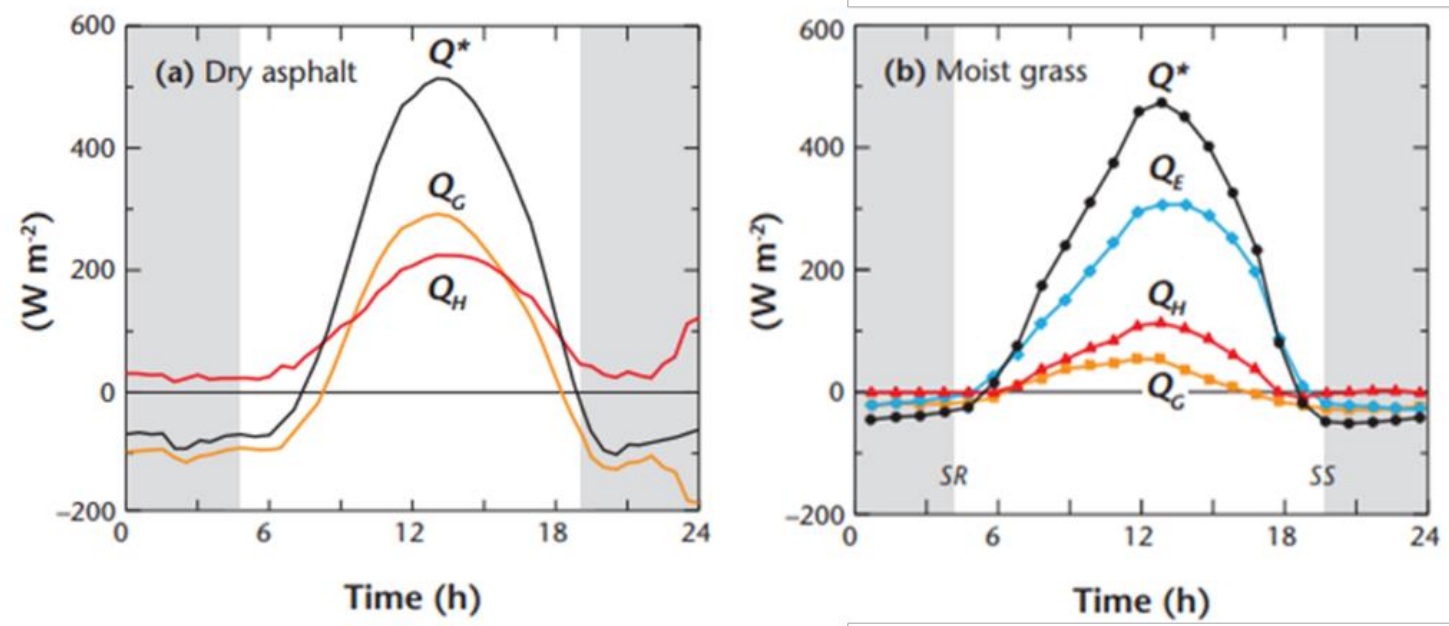
\includegraphics[trim={0 0 0 0},clip,scale=0.8]{SEB.png}
%\caption{\bf Example surface energy balances of (a) dry asphalt road and (b) moist grass in an urban park (b), taken from \cite{Oke2017}.}
% \label{fig:7.1}
%\end{figure}
%
%Impervious surfaces also typically absorb large amounts of \gls{Qstar} during the day \citep{Cohard2018}. This accumulated $\Delta$\gls{Qs} is then released at night, which can support a positive night-time \gls{Qh} (Figure \ref{fig:7.1}) \citep{Oke2017,Cohard2018}. Consequently, urban areas are prone to high night-time temperatures, which in turn, can led to negative health outcomes \citep{Clarke1972,Coutts2010}. 
%
%Water on impervious surfaces introduces \gls{Qe} into the energy balance and modifies the distribution of energy. However, \gls{Qe} is closely related to how water behaves on impervious surfaces. This is explored in the next section.
%
%\subsubsection{Impervious Surface Hydrology}\label{sec:appendix7.1.3}
%As with energy, it is beneficial to start with the water balance to investigate impervious surface hydrology. The urban energy and water balance are linked as \gls{Qe} is directly related to evaporation (\gls{E}). The urban energy balance is given by:
%
%\begin{equation}
%P + I = E + D + R + \Delta S
%\label{eq:7.2} 
%end{equation}
%
%where \gls{P} is precipitation, \gls{I} is non-natural water inputs (i.e., pavement watering), \gls{D} is drainage (also referred to as infiltration), \gls{R} is runoff, and $\Delta$S is change in surface storage \citep{Grimmond1986,Mitchell2008}.
%
%Accurately estimating these terms is difficult, as the hydraulic behaviour of urban surfaces is highly variable. It is dependent on the specific surface characteristics, the intensity and duration of rainfall \citep{Fletcher2013}, and can vary on seasonal and decadal timescales \citep{Redfern2016}.
%
%In this review, we are specifically interested in the behaviour of water on impervious surfaces. Thus, the next sections will explore how each term on the right-hand side of Equation \ref{eq:7.2} behaves within this context.
%
%\subsubsection{Evaporation}\label{sec:appendix7.1.3.1}
%
%Evaporation on impervious surfaces is intermittent, and generally only accounts for a minor portion of total evapotranspiration in urban areas. However, this portion can still be significant. For example, \cite{Ramamurthy2014} used the Princeton Urban Canopy Model (PUCM) and observations to analyse \gls{Qe} during a 10-day period with relatively high rainfall. During this studied period, it was found that the \gls{Qe} from rooftops, concrete, and asphalt surfaces contributed to 17\% of total \gls{Qe}.
%
%Evaporation is dependent on various factors. These factors are summarised by \cite{Monteith1991} as follows: the net available energy, the state of the surrounding air, and the available water on the evaporating surface. The net available energy relates to the energy balance (Equation \ref{eq:7.1}), where \gls{Qstar} is commonly the major energy source for evaporation \citep{Penman1948,McMahon2013}.
%
%On the other hand, the state of the surrounding air relates to its temperature, vapour pressure, and its velocity \citep{McMahon2013}. These factors are not independent, as the maximum saturation of water vapour in the air varies with temperature, with higher temperatures having a higher saturation. Temperature also has a slight effect on the amount of energy required for evaporation (i.e., the latent heat of vaporisation), which is lower for higher temperatures \citep{Shuttleworth2012}. Vapour pressure relates to the actual amount of water vapour in the air compared to the amount at saturation and influences the evaporation rate. Velocity corresponds to the removal of water vapour from the evaporating surface, which is needed for evaporation to occur (McMahon et al. 2013).
%
%Finally, evaporation is also highly dependent on the amount of water available. Thus, we need to know how water is distributed on impervious surfaces, i.e., the remaining terms in the urban water balance.
%
%\subsubsection{Drainage}\label{sec:appendix7.1.3.2}
%
%Drainage is generally less substantial in urban settings compared to rural areas; however, it is highly variable spatially and temporally \citep{Raimbault2001}. It is often incorrectly assumed that constructed urban surfaces, such as roads and pavements, are completely impermeable and thus have no infiltration \citep{Redfern2016}. Indeed, the term 'impervious' is perhaps misleading when drainage through these surfaces has been observed and measured (see \cite{Rammal2020} and \cite{Redfern2016}).
%
%Infiltration is dependent on the amount of void space within a material, as it dictates the amount of water that can pass through \citep{Aboufoul2017}. Factors that also impact infiltration include the surface storage, surface properties, age, traffic loading, cracks, and joints \citep{Redfern2016,Rammal2020}. For example, \cite{Ramier2004} tested the hydrological behaviour of three asphalt concrete samples, one of which was taken from a heavy traffic simulator, and thus was more porous due to deterioration. For the deteriorated sample, 58\% of the rainfall over a 5-month period infiltrated, compared to 2 to 3\% infiltration of the other samples. Thus, infiltration is difficult to accurately predict.
%
%\subsubsection{Storage and Runoff}\label{sec:appendix7.1.3.3}
%
%The water storage capacity of impervious surfaces controls the water balance. It dictates the amount of water that is available for evaporation or infiltration, and what will be lost to runoff.
%
%The bucket model (also known as the water reservoir model) is commonly employed for impervious surfaces. This involves assuming surfaces have a variable water storage with a fixed upper limit, which once exceeded, generates runoff \citep{Rammal2020}. Traditionally, urban areas are designed to remove excess water as quickly as possible via pathways such as sewer systems. Thus, it is a common to assume that runoff from impervious surfaces is transported out of the system (e.g., \cite{Kronaveter2001}).
%
%As with drainage, the maximum water storage of urban surfaces is highly heterogeneous. Influencing factors include surface type, geometrical characteristics, slope, and the rainfall event \citep{Rammal2020}. One study investigated water holding depths for brick, asphalt, cement, and concrete surfaces and found variation from 0.4 to 1mm (Figure \ref{fig:7.2}), with larger roughness correlated with higher interception \citep{Zhou2021a}.
%
%\begin{figure}
%\centering
%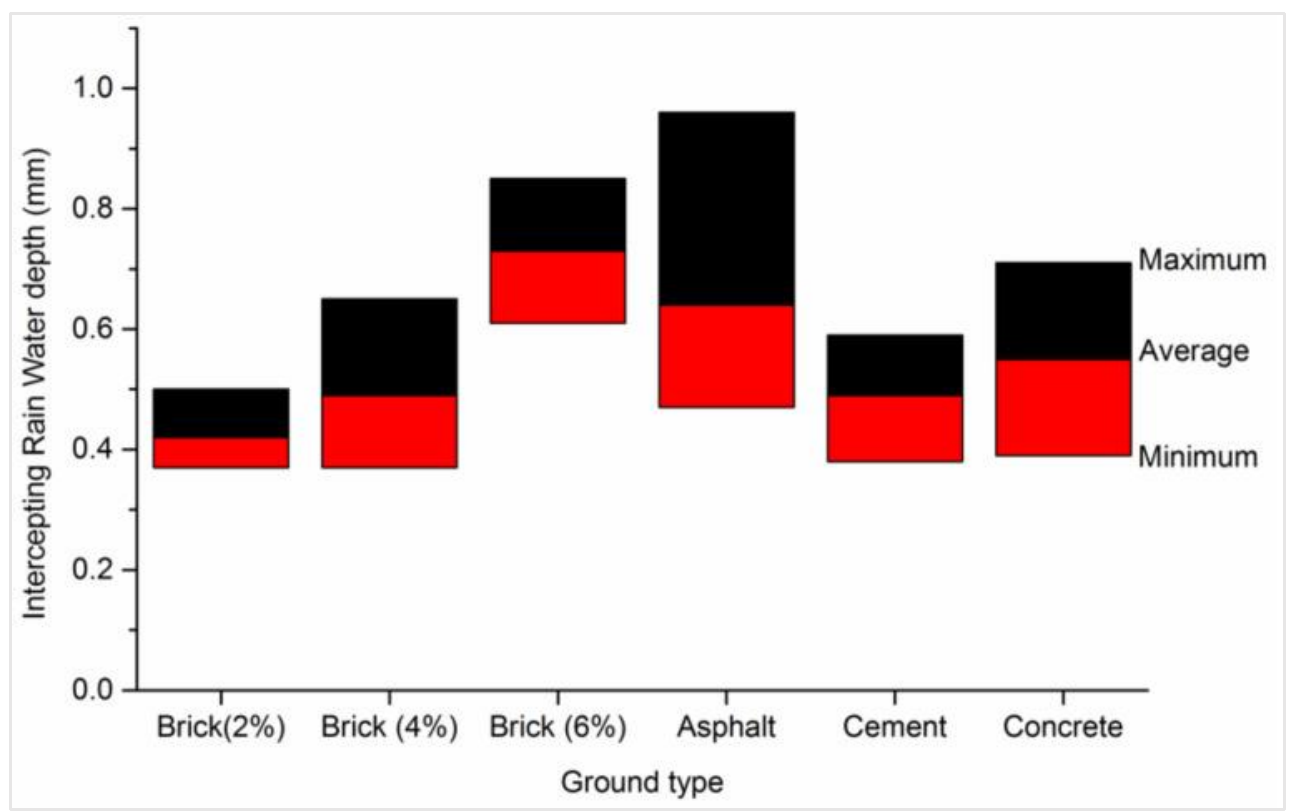
\includegraphics[trim={0 0 0 0},clip,scale=0.7]{Impervious.png}
%\caption{\bf Experimental results of impervious surfaces maximum storage capacity, taken from \cite{Zhou2021a}.}
% \label{fig:7.2}
%\end{figure}
%
%This maximum water storage strongly impacts the amount of evaporation, and this is important to be aware of \citep{Wouters2013}. We have established that impervious surfaces have limited water storage, and may be prone to drainage, however evaporation, and thus \gls{Qe}, can still be a significant factor from these surfaces. In the next section, we introduce an urban heat mitigation technique that makes use of this: pavement watering.
%
%\subsubsection{Pavement Watering}\label{sec:appendix7.1.4_}
%
%Pavement watering describes the practise of wetting otherwise dry impervious surfaces, often roads and footpaths, on hot days. The subsequent evaporation from these wet surfaces induces a cooling effect, and thus has potential to mitigate urban heat. There is also a slight benefit associated with runoff transporting warmed water out of the system \citep{Hendel2020}. This technique can include engineered permeable surfaces designed to retain water; however, this is considered out of scope for this research. The benefits of this strategy have been investigated through field and modelling experiments. The following sections will explore these two approaches.
%
%\paragraph{Field Experiments}\label{sec:appendix7.1.4.1}
%
%Pavement watering has been adopted in France, Japan, and Korea in response to excess urban heat. Since 2013, pavement watering has been conducted every summer in Paris when certain meteorological conditions, relating to the city's heat health warning thresholds \citep{Pascal2006}, are met (Table \ref{table:7.1}). Non-potable water is deposited with a cleaning truck at set intervals or via a removable water pipe which continuously supplies water. These events have been extensively studied to characterise the surface and subsurface pavement temperature changes \cite{Hendel2015,Hendel2015a,Hendel2015b,Hendel2014}, as well as to investigate the climate benefits \citep{Hendel2016,Parison2020}.
%
%
%\begin{table}[!ht]\caption{Weather conditions for pavement watering used in Paris, corresponding to relaxed heatwave conditions, taken from \cite{Hendel2015a}.}
%    \centering
%    \begin{tabular}{|p{5.0cm}|p{5.0cm}|p{5.0cm}|}
%    \hline
%        \textbf{Parameter} & \textbf{Pavement watering conditions} & \textbf{Heat-wave warning level}\\ \hline
%		Mean 3-day minimum air temperature (BMI$_{Min}$)&$>$16$^{\circ}$C & $>$21$^{\circ}$C\\ \hline
%		Mean 3-day maximum air temperature (BMI$_{Max}$)&$>$25$^{\circ}$C & $>$31$^{\circ}$C\\ \hline
%		Wind speed &$<$10 km h$^{-1}$ &-\\ \hline
%		Sky conditions&Sunny (less than 2 oktas cloud cover) &-\\ \hline  
%    \end{tabular} \label{table:7.1}
%\end{table}
%
%
%In Japan, pavement watering is tied to a 17th century Japanese custom, uchimizu, where water is sprinkled on streets outside houses and shops. Due to the cooling benefits, the practice is currently encouraged by Japanese authorities \citep{Solcerova2018}. Pavement watering has also been utilised at a larger scale, using existing snow-melting pipe networks to wet roads in the summer \citep{Kinouchi1997,Himeno2010}.
%
%In Korea, pavement watering is known as `Clean Road'. Clean Road systems are installed along various roads in Korea, where water is discharged for a range of reasons, including to provide cooling in excessive heat and melt snow in winter \citep{Na2021}. For example, the Clean Road system in Daegu utilises underground water discharged from a subway station to water approximately 9.1km of road two times per day in summer, and three times in case of extreme heat \citep{Kim2015,Na2021}.
%
%The measured benefits of pavement watering are summarised in Table \ref{table:7.2}. The maximum changes in air temperature and relative humidity range from 0$^{\circ}$C to -4$^{\circ}$C and 0\% to +4.08\% respectively. Thermal comfort benefits are of a higher magnitude than air temperature changes, as the former considers mean radiant temperature, and thus also accounts for reductions in surface temperature (Table \ref{table:7.2}).


\subsection{Previous pavement watering experiments}\label{sec:appendix7.1}
\begin{table}[!ht]\caption{Observed maximum impacts of pavement watering field experiments. GT is Globe Temperature, \gls{utci} is Universal Thermal Climate Index, and SET* is Standard New Effective Temperature.}
    \centering
    \footnotesize
    \begin{tabular}{|p{2.0cm}|p{1.5cm}|p{6.0cm}|p{1.5cm}|p{1.0cm}|p{1.7cm}|}
    \hline
        \textbf{Study} & \textbf{Measurement Height (m)} &\textbf{Details} & \textbf{Air Temperature ($^{\circ}$C)} &\textbf{Humidity (\%)} &\textbf{Measure of Thermal Comfort ($^{\circ}$C)}\\ \hline
        \cite{Kinouchi1997}&1&Snow-melting pipes, watering road from 10:00 to 14:00 &-1 &+4 &-4 (GT) \\ \hline
        \cite{Himeno2010}&0.9&Snow-melting pipes, 12L min$^{-1}$ on road for 3 min every 30 min Morning: 8:30 to 10:30 &-2 &-& - \\ \hline       
        \cite{Himeno2010}&0.9&Snow-melting pipes, 12L min$^{-1}$ on road for 3 min every 30 min Afternoon: 17:10 to 19:10 &-4 &-& - \\ \hline  
        \cite{Hendel2016}&1.5&Paris 2013-2014 summer field experiments
        Louvre site: cleaning truck and a manual operator for road and
        sidewalk 1 mm every hour from 6:20 to 11:30 and every 30
        min from 14:00 to 20:30 &-0.79 &+4.1 &-1.03 (\gls{utci}) \\ \hline
         \cite{Hendel2016}&1.5&Belleville site: 40m watering pipe continuously watered pavement at 25mm h$^{-1}$ from 7:00 to 21:00 &-0.60 &+1.6 &-0.93 (\gls{utci}) \\ \hline         
        \cite{Parison2020}&1.5&Paris annual summer field experiments, statistical analysis of Louvre site data: 2013-2015 campaign, watering road and sidewalk (100\% of street width)  &-1.02 &+4.08 &-1.93 (\gls{utci}) \\ \hline
		\cite{Parison2020}&1.5&2016-2018 campaign, watering road only (66\% of street width)&-0.97 &+3.03 &-3.42 (\gls{utci}) \\ \hline
        \cite{Takebayashi2021}&1.2&Sufficient water supplied to wet the surface watering one road lane&None\tablefootnote{\label{none}As only one of multiple lanes were watered, no change in air temperature and relative humidity was observed at 1.2m, presumed to be due to air mixing} &None$^{1}$ &-0.8 (SET*) \\ \hline
         \cite{Takebayashi2021}&1.2&Watering pedestrian pavement&- &- &-2.5 (SET*) \\ \hline
    \end{tabular} \label{table:7.2}
\end{table}

%These maximum benefits are measured next to or on top of watered surfaces, where impacts are greatest. The extent of cooling was investigated by \cite{Takebayashi2021}, who found that thermal comfort benefits reduce the greater the distance from the wetted surface and the smaller the reduction in surface temperature. For example, the reduction in Standard New Effective Temperature (SET*) decreased from 0.48$^{\circ}$C to 0.24$^{\circ}$C 1m away from the watered roadway, for a 7.4$^{\circ}$C reduction in surface temperature.
%
%These studies highlight that the advantage of pavement watering lies in its accessibility to highly urbanised areas and quick cooling response. One study also found a reduction of 5\% to 15\% of fine dust when comparing a watered road to a non-watered area, suggesting that pavement watering may reduce air pollution \citep{Kim2014a}. On the other hand, pavement watering is constrained by localisation of cooling benefits, water availability, and required frequency of watering due to the limited water storage capacity of surfaces. Thus, optimising pavement watering to maximise water efficiency and cooling benefit is important.
%
%\cite{Hendel2020} summaries the general conditions to maximise pavement watering efficiency: the surface is fully exposed to sunlight and enough water is applied to prevent the surface drying while also minimising runoff and drainage, i.e., optimising for evaporation and thus \gls{Qe}.
%
%The discussed experimental studies provide a basis for pavement watering; however, it is clear that results depend on the specific site locations and prevailing conditions. Indeed, \cite{Hendel2016} notes that a limitation of field studies is the assumption that control and experimental sites are comparable. Pre-existing differences and interactions between sites may cause errors in reported cooling effects, although there have been some attempts to overcome this issue with statistical analysis.
%
%\paragraph{Modelling Experiments}\label{sec:appendix7.1.4}
%
%Models provide an alternative method to investigate pavement watering. They overcome the need for a comparable control and experimental site. Models also allow for more experimental control and are generally less demanding than observational measurements, although they rely on imperfect abstractions of the real world \citep{Krayenhoff2021}.
%
%One such experiment utilises the Town Energy Balance (TEB), a mesoscale urban canopy model, to simulate a 2100 heatwave in Paris \citep{Daniel2018}. Pavement watering was found to induce a cooling of up to 1$^{\circ}$C for air temperature at 2m when simulated from 8am to 8pm, with 603km$^{2}$ surfaces being wetted at 1.5GL day$^{-1}$. 
%
%\cite{Broadbent2018b} also investigated the cooling benefits of irrigation using TEB (embedded in SURFEX, a land surface modelling scheme), although watering was only simulated on pervious surfaces. Bare soil irrigation was found to have the greatest irrigation efficiency (in terms of cooling benefit per volume of water). For this reason, impervious surfaces can also be an effective cooling method in built-up areas.
%
%\subsubsection{Summary}\label{sec:appendix7.1.5}
%Excess heat in urban areas will be further exacerbated by climate change and increasing urbanisation. Impervious surfaces contribute to this heat, as they partition a large proportion of energy into the sensible heat flux while limiting the latent heat flux. The lack of evaporative cooling from these surfaces is due to the lack of water, which is driven by their limited water storage capacity. However, evaporation, and thus latent heat flux, can be favoured by adding water, and avoiding water loss to drainage and runoff, especially in conditions which optimise evaporation.
%
%Pavement watering is an urban heat mitigation technique that attempts to do this by watering impervious surfaces on hot days. Various field studies in France, Japan, and Korea have shown that the technique reduces air temperature and improves thermal comfort. However, pavement watering has yet to be explored in an Australian context. This literature review was done to inform a study on pavement watering in Melbourne, Australia.

\subsection{Daily Weather Observations}\label{sec:appendix7.2}

\begin{table}[!ht]\caption{The daily weather observations for Melbourne, Victoria for the experiment days in February 2022, taken from \cite{BOM2022}.}
    \centering
    \begin{tabular}{|p{0.6cm}|p{0.6cm}|p{0.6cm}|p{0.6cm}|p{0.6cm}|p{0.6cm}|p{0.6cm}|p{0.8cm}|p{0.6cm}|p{0.6cm}|p{0.6cm}|p{0.6cm}|p{0.8cm}|p{0.6cm}|}
    \hline 
        &Min.&Max.&Daily&9am&9am&9am&9am&9am&3pm&3pm&3pm&3pm&3pm\\  
        Date & \gls{ta} & \gls{ta} & Rain & \gls{ta} & \gls{rh} & Cld\tablefootnote{\label{cld}Fraction of sky obscured by cloud} & Wind Dir. & Wind & \gls{ta} & \gls{rh} & Cld & Wind Dir. & Wind \\          
        ~ &$^{\circ}$C &$^{\circ}$C & mm &$^{\circ}$C & \% & oktas &~ & km/h &$^{\circ}$C & \% & oktas &   ~& km/h  \\ \hline
        7th & 14.7 & 28.6 & 0 & 20.3 & 58 & 1 & NE & 7 & 27.2 & 40 & 1 & S & 13 \\ \hline
        8th & 15.4 & 30.5 & 0 & 20 & 60 & 1 & NNE & 9 & 30 & 31 & 3 & NE & 6 \\ \hline
        12th & 15.7 & 28.3 & 0 & 18.7 & 68 & 1 & ESE & 6 & 26.6 & 47 & 2 & SSW & 7 \\ \hline
        13th & 17.1 & 32.1 & 0 & 23.5 & 50 & 4 & NNW & 20 & 30.3 & 34 & 7 & NNW & 20 \\ \hline
    \end{tabular}\label{table:7.3}
\end{table}




\subsection{Sensor Validation and Corrections}\label{sec:appendix7.3}

Figure \ref{fig:7.3} shows the validation period for \gls{ta} and \gls{rh}. \gls{ta} was discarded in favour of $T_{p,1.5}$ as both measured air temperature at 1.5m, as there were clear issues with the control \gls{ta} sensor. The mean difference between \gls{rh} control and experimental sensors from this validation period was calculated (2.5\%) and used to correct the experiment data.

\begin{figure}
\centering
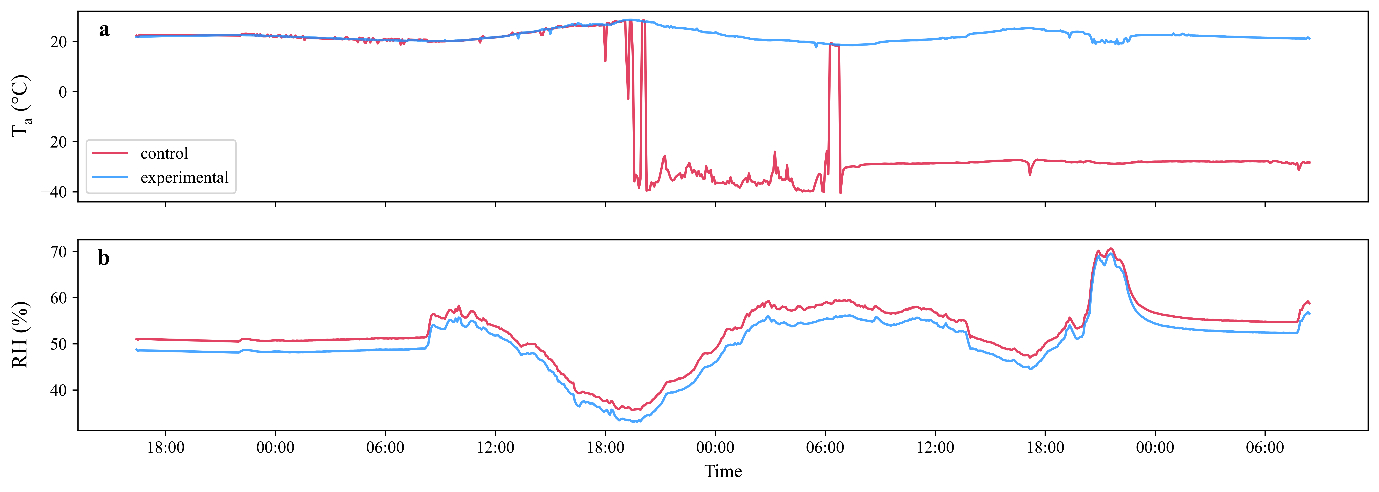
\includegraphics[trim={0 0 0 0},clip,scale=1.0]{pict018.png}
\caption{\bf The results from validation period (25th to 28th of Feb 2022) for the (a) \gls{ta} and (b) \gls{rh} sensors.}
 \label{fig:7.3}
\end{figure}

Figure \ref{fig:7.4} shows the validation period for the Kestrels (\gls{Kt} and \gls{Krh}). \gls{Kt} was considered reasonable, while the mean difference between \gls{Krh} sensors from this validation period was calculated (3.8\%) and applied to experiment data.

\begin{figure}
\centering
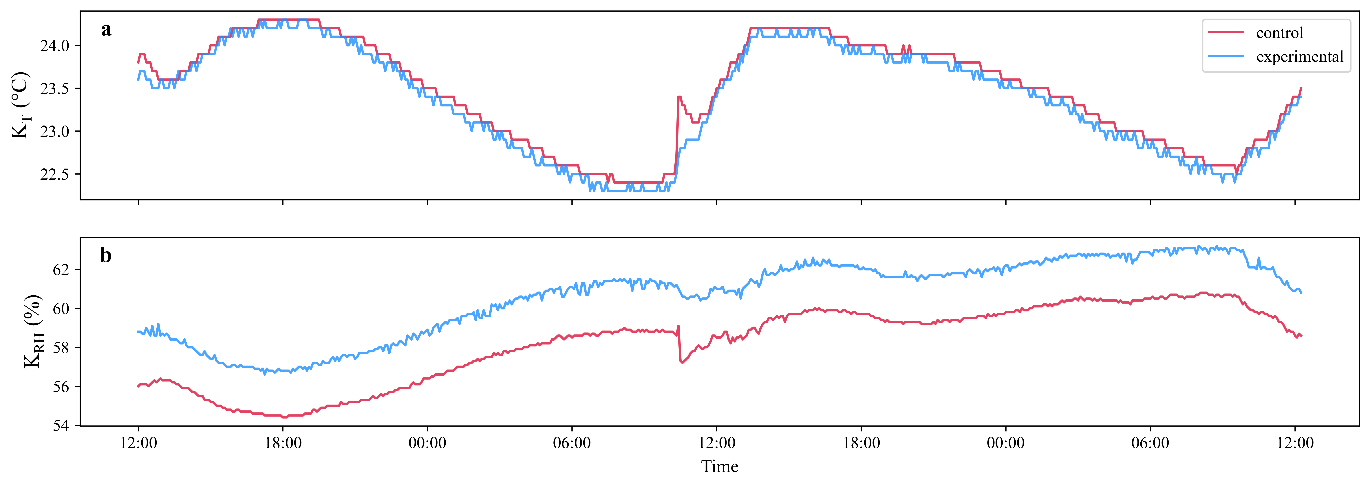
\includegraphics[trim={0 0 0 0},clip,scale=1.0]{pict019.png}
\caption{\bf The results from validation period (15th to 17th of Feb 2022) for the Kestrels (a) \gls{Kt} and (b) \gls{Krh} sensors.}
 \label{fig:7.4}
\end{figure}

Figure \ref{fig:7.5} shows the validation period for the \gls{tg}, \gls{Kdown}, \gls{Kup}, \gls{Ldown}, and \gls{Lup}. The \gls{tg}, \gls{Kdown}, and \gls{Kup} was considered reasonable, while \gls{Ldown} and \gls{Lup} were not comparable.

\begin{figure}
\centering
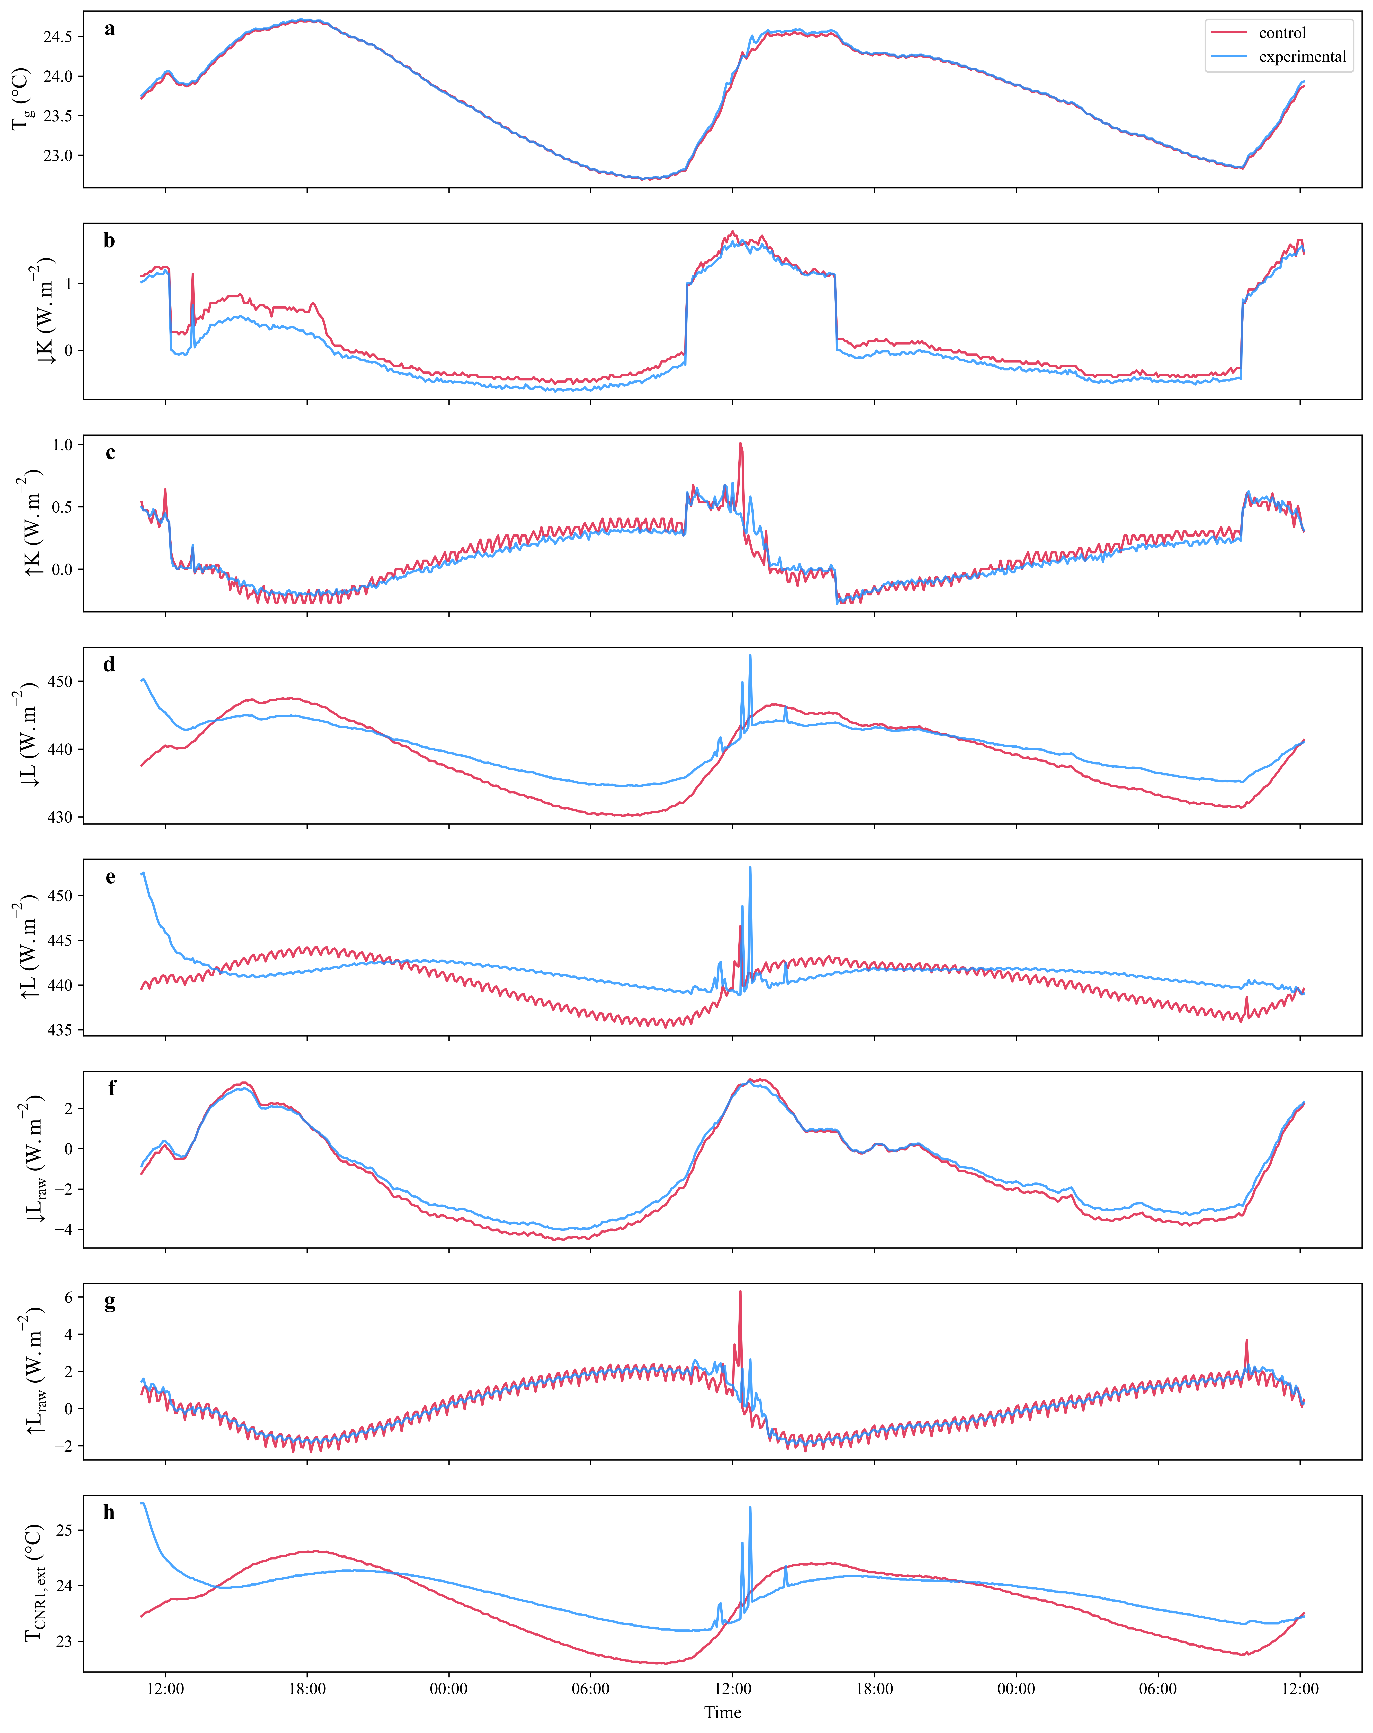
\includegraphics[trim={0 0 0 0},clip,scale=1.0]{pict020.png}
\caption{\bf The results from validation period (15th to 17th of Feb 2022) for the (a) \gls{tg}, (b) \gls{Kdown}, (c) \gls{Kup}, (d) \gls{Ldown}, (e) \gls{Lup}, (f) \gls{Ldown}$_{raw}$, (g) \gls{Lup}$_{raw}$, and (h) \gls{tcnr1}$_{,ext}$ sensors.}
 \label{fig:7.5}
\end{figure}

The CNR1 measures the exchange of thermal radiation between the sensor and the object being faced ($L_{raw}$), which is then used alongside the temperature of the CNR1 (\gls{tcnr1}) to calculate $L$ as follows:

\begin{equation}
L = L_{raw} + \sigma (T_{CNR1} + 273.15)^{4}
\label{eq:7.3} 
\end{equation}

where $\sigma$ is the Stefan-Boltzmann constant (5.67 $\times 10^{-8} Wm^{-2}K^{-4}$) \citep{CampbellScientific2011}.

Type E thermocouples were attached to the bottom of the CNR1 sensors to measure its temperature (\gls{tcnr1}$_{,ext}$) instead of the CNR1 internal temperature sensors (\gls{tcnr1}$_{,int}$) due to limited inputs on the data loggers. It can be seen that the \gls{tcnr1}$_{,ext}$, not the \gls{Ldown}$_{raw}$, \gls{Lup}$_{raw}$ (Figure \ref{fig:7.5}) was causing the difference between control and experimental $L$. 

Additional investigation found that the internal temperature of the control and experimental CNR1 do not vary significantly (Figure \ref{fig:7.6}), and thus it is likely that one or both of the thermocouples were not placed appropriately and/or securely on the CNR1. Therefore, the assumption was made that the actual \gls{tcnr1} did not vary between the control and experimental sensors. Thus, \gls{Ldown} and \gls{Lup} was corrected with calculations based on the same CNR1 temperature.

\begin{figure}
\centering
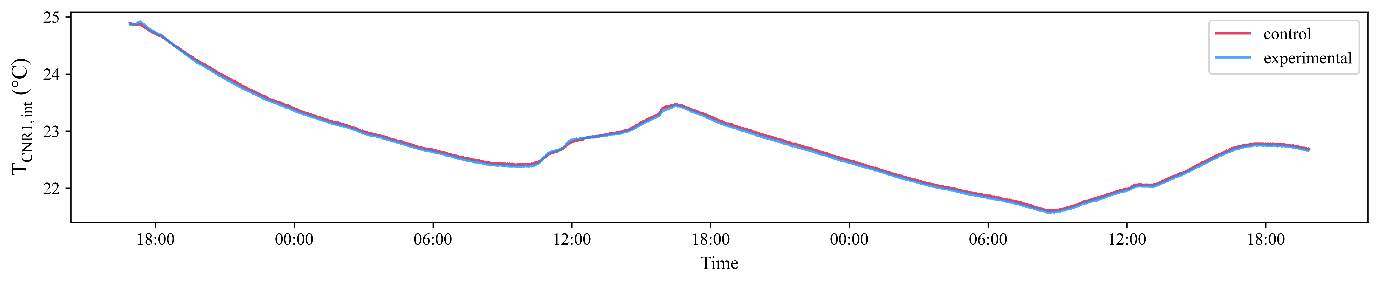
\includegraphics[trim={0 0 0 0},clip,scale=1.0]{pict022.png}
\caption{\bf The results from validation period (28th to 30th of Mar 2022) for the \gls{tcnr1}$_{,int}$ sensors.}
 \label{fig:7.6}
\end{figure}


The control \gls{tcnr1}$_{,ext}$ was identified as the `correct' temperature was based on deriving the surface temperature (\gls{tsdrvd}) (see \ref{sec:appendix7.4.2}).



\subsection{Derived Variables}\label{sec:appendix7.4}
\subsubsection{Wind Speed 10m}\label{sec:appendix7.4.1}

It should be noted that the wind profile of the atmospheric boundary layer is generally logarithmic, and thus is commonly approximated using the log wind profile equation \citep{Banuelos-Ruedas2010}. However, this requires the surface roughness and atmospheric stability to be known. Thus, to avoid assumptions and uncertainties associated with these variables, and as wind was measured at two heights, the wind profile power law (also known as the Hellmann exponential law) was used. This is commonly used when information is limited, although it is less theoretically accurate \citep{Banuelos-Ruedas2010}.

The wind profile power law is defined as:

\begin{equation}
u_{2} = u_{1}  { \bigg( \frac{ z_{2} }{ z_{1} } \bigg) } ^{\alpha}
\label{eq:7.4}
\end{equation}


where $u_{1}$ and $u_{2}$ is wind speed ($ms^{-1}$) at height $z_{1}$ and $z_{2}$(m) respectively, and $\alpha$ is the wind shear exponent \citep{Manwell2010}. Firstly, $\alpha$ was derived from measured wind speed at 0.3m (\gls{Ku}) and 2.25m (\gls{u}). The average of the control and experimental \gls{Ku} values was used as it is assumed that the wind speed was the same for the control and experimental sites, as they were within 10m of each other. The average $\alpha$ was then used to calculate wind speed at 10m (\gls{u10}). See Figure \ref{fig:7.7} for the daily measured and derived wind speeds.

\begin{figure}
\centering
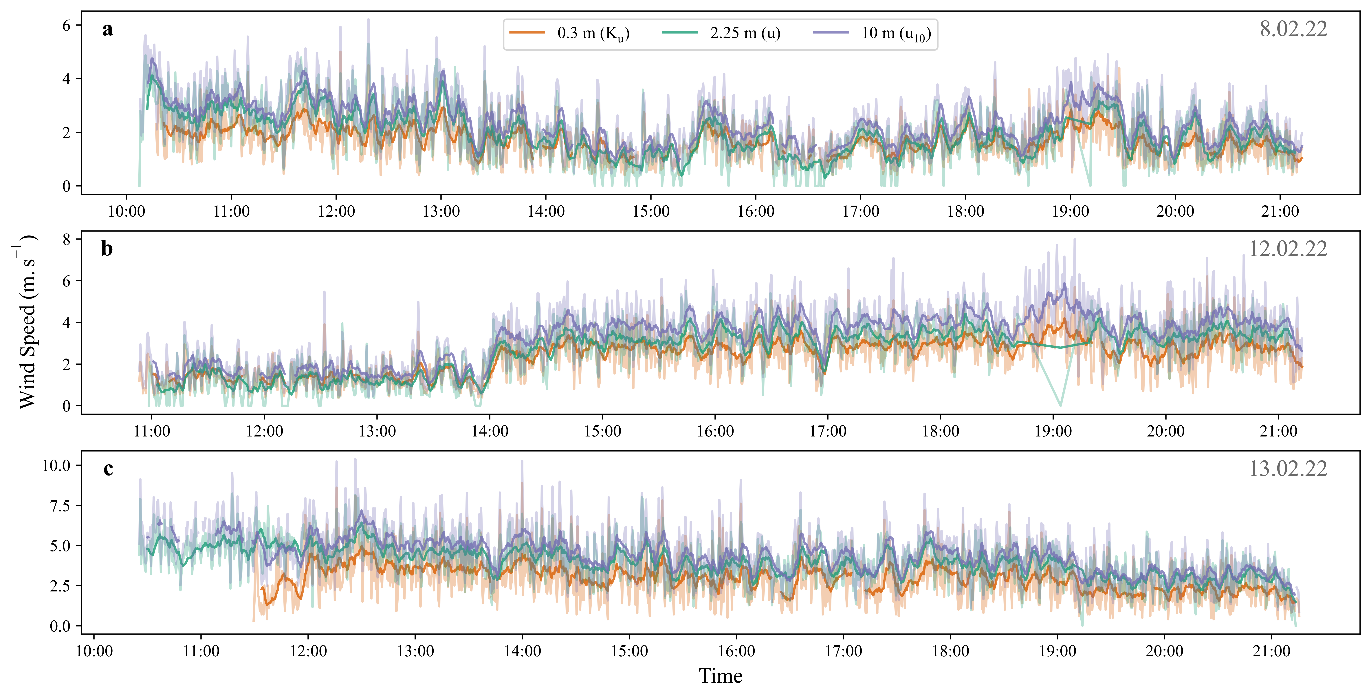
\includegraphics[trim={0 0 0 0},clip,scale=1.0]{pict024.png}
\caption{\bf Wind speeds at different heights for the experiment days: (a) 8th, (b) 12th, (c) 13th. The transparent lines are the raw data, while the solid lines are the 5-minute running average.}
 \label{fig:7.7}
\end{figure}



\subsubsection{Surface Temperature}\label{sec:appendix7.4.2}

Only the experimental station had a surface temperature sensor (\gls{ts}) (Figure \ref{fig:2.1}), thus surface temperature was derived for the control and experimental station (\gls{tsdrvd}), the latter for verification and consistency. \gls{Lup}($Wm^{-2}$) and \gls{ts}($^{\circ}$C) are related to each other by the following equation:

\begin{equation}
L\uparrow = \epsilon \sigma (T_{s} + 273.15)^{4} + (1 - \epsilon) L\downarrow
\label{eq:7.5}
\end{equation}

where $\sigma$ is the Stefan-Boltzmann constant (5.67 $\times 10^{-8} Wm^{-2}K^{-4}$) and $\epsilon$ is emissivity of the surface (-). The magnitude of $\epsilon$ is unknown, but for road surfaces is commonly above 0.85 \citep{Oke2017}. Assuming that the surface is a black body (i.e., $\epsilon$ = 1) and rewriting to solve for \gls{tsdrvd} simplifies the equation to:

\begin{equation}
T_{s,drvd} =  { \bigg( \frac{  L\uparrow } {\sigma}   \bigg) }^{0.25} - 273.15
\label{eq:7.6}
\end{equation}

As \gls{Lup} was found to impacted by errors associated with \gls{tcnr1} (\ref{sec:appendix7.3}), \gls{Lup} was calculated using both the control and experimental \gls{tcnr1} (Equation \ref{eq:7.3}) before being used to calculate \gls{tsdrvd} (Equation \ref{eq:7.6}). Comparing the experimental \gls{tsdrvd} with measured \gls{ts} showed that the black body assumption is flawed (Figure \ref{fig:7.8}). To overcome this, the terms ignored in Equation \ref{eq:7.6} were indirectly accounted for by performing a linear regression between \gls{ts} and \gls{tsdrvd} and applying this calculated linear model for each experiment day.

The results of the different methods to calculate experimental \gls{tsdrvd} alongside measured \gls{ts} are shown in Figure \ref{fig:7.8}. It is clear that the \gls{tsdrvd} computed with linear model using the \gls{Lup} calculated with the control \gls{tcnr1} replicates the measured \gls{ts} well. This is also shown as this method had the best performing \gls{r2} values, which were 0.98, 0.98, and 0.96 for the 8th, 12th, and 13th respectively. This implies that the control \gls{tcnr1} captured the `correct' temperature of the CNR1 sensor, while the experimental \gls{tcnr1} sensor may have been in an incorrect position.


\begin{figure}
\centering
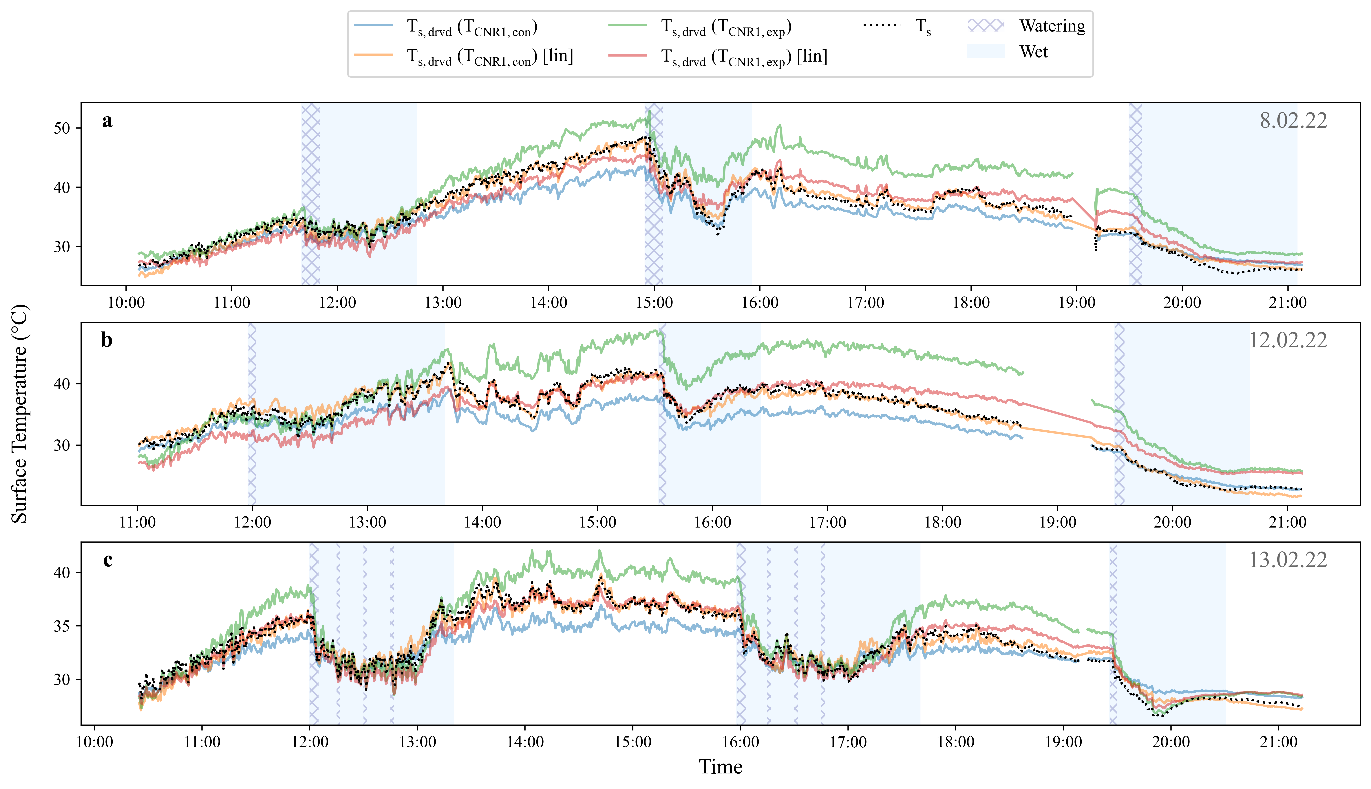
\includegraphics[trim={0 0 0 0},clip,scale=1.0]{pict027.png}
\caption{\bf Different methods to derive surface temperature (\gls{tsdrvd}) for the experimental site compared to measured (\gls{ts}) for the experiment days: (a) 8th, (b) 12th, (c) 13th.}
 \label{fig:7.8}
\end{figure}

\gls{tsdrvd} was then calculated for the control station using the calculated linear model along with \gls{Lup} calculated with the control \gls{tcnr1} (Figure \ref{fig:7.17} and Table \ref{table:7.5}). For consistency, \gls{tsdrvd} was used for both the control and experimental surface temperature to interpret impacts of watering, rather than \gls{ts}.

\subsubsection{Vapour-Pressure Deficit}\label{sec:appendix7.4.3}

Instead of \gls{rh}, a more accurate way to express the driving force of water loss is vapour-
pressure deficit (\gls{vpd}). \gls{vpd} (kPa) is defined as the difference between the saturated
vapour pressure ($e_{s}$ , kPa) and the ambient vapour pressure ($e_{a}$, kPa).
The $e_{s}$ can be calculated as:

\begin{equation}
e_{s} = a e^{\bigg(  \frac{  bT_{p,1.5}   }{ T_{p,1.5} + c }    \bigg)}
\label{eq:7.7}
\end{equation}

where a, b, and c are constants. As suggested by \cite{McMahon2013}, constants defined by \cite{Allen1998} are used (a = 0.6108 kPa, b = 17.27, c = 237.3$^{\circ}$C). Relative humidity (\gls{rh},\%) is the vapour pressure ratio, and thus \gls{vpd} can be written as:

\begin{equation}
VPD=e_{s}\bigg( 1 - \frac{RH}{100} \bigg)
\label{eq:7.8}
\end{equation}

$T_{p,1.5}$ and \gls{rh} from the control and experimental stations (Figure \ref{fig:2.1}) were used to calculate \gls{vpd}. As the $T_{p,1.5}$ was not working for the majority of experiment 13M, \gls{vpd} could not be calculated for this experiment, however, it can be assumed it was quite high given the other \gls{vpd} values on the 13th.


\subsubsection{Mean Radiant Temperature and the Universal Thermal Climate Index}\label{sec:appendix7.4.4}

To calculate the mean radiant temperature (\gls{Tmrt}, K), the pythermalcomfort python package was used \citep{Tartarini2020}. This employs the formula specified by ISO 7726:1998 Standard. Firstly, the heat transfer coefficient ($h$) is calculated as the maximum value between natural and forced convection as follows:

\begin{equation}
h = max \begin{cases}  \frac{  1.4 \cdot |tg-tbd|^{0.25} }{d} \\  6.3 \frac{v^{0.6}}{d^{0.4}} \end{cases}
\label{eq:7.9}
\end{equation}

where $tg$ is global temperature (K), $tdb$ is air temperature (K), $v$ is the wind speed (ms$^{-1}$), and $d$ is the diameter of the globe (m). \gls{Tmrt} can then be calculated as follows:

\begin{equation}
T_{MRT}=  {  \bigg( tg^{4} + h \frac{tg - tbd}{\epsilon \cdot 5.67\times 10^{-8}} \bigg)}^{0.25}
\label{eq:7.10}
\end{equation}

where $\epsilon$ is the emissivity of the globe.

The library pythermalcomfort facilitated the conversion of units, thus \gls{tg}, $T_{p,1.5}$, and \gls{u10} were used to calculate \gls{Tmrt}. For the globe diameter and emissivity, Campbell Scientific BlackGlobe values of 0.152 m and 0.957 respectively were used \citep{CampbellScientific2022}. \gls{Tmrt} was also converted to$^{\circ}$C.

The same python library was used to calculate the Universal Thermal Climate Index (\gls{utci},$^{\circ}$C), a mathematical model that assesses the outdoor thermal environment and provides an indicator for heat stress. The model requires $T_{p,1.5}$ , \gls{Tmrt}, \gls{u10} ($ms^{-1}$), and \gls{rh} (\%).



\subsubsection{Surface Energy Balance}\label{sec:appendix7.4.5}

Latent heat flux (\gls{Qe}, $Wm^{-2}$) was calculated as:

\begin{equation}
Q_{e} = \ell _{v} \rho_{w} \frac{V}{A} \frac{1}{t} \frac{1m}{1000mm}
\label{eq:7.11}
\end{equation}

where $\ell _{v}$ is the latent heat of vaporisation (2.5$\times$10$^{6}$ J kg$^{-1}$), $\rho_{w}$ is the density of water (1000 kg m$^{-3}$), $V$ is the volume of water (L), $A$ is the area watered (10m$\times$10m), $t$ is the total time to evaporate (seconds), and the last term converts the units to $Wm^{-2}$. The $t$ was taken as the time it took for the area under the experimental station to become dry after watering.

The $V$ was adjusted to take into account water accumulation on the edge of the watered plot and losses due to runoff, based on observations. The carpark was slightly sloped towards the edges, and despite efforts to contain water inside the established plot, there was significant build up along the west edge and varying amounts of runoff (Figure \ref{fig:2.1}, Table \ref{table:2.2}). It was assumed that there was no drainage, as the surface did not appear to have any cracks and any infiltration was considered negligible. It was also assumed that the water storage capacity of the plot was 40L when subtracted for runoff and edge build up, and thus V = 40L was used to calculate \gls{Qe}. For the experiments where 20L was added after the initial watering at set intervals (13M and 13A), as this water was added to the east side of the plot and resulted in no observable extra runoff or build-up, 40L from the initial 60L was added to the following 20 L (i.e., $V$ = 100L).

To calculate sensible heat flux (\gls{Qh}, $Wm^{-2}$), the following formula was used:

\begin{equation}
Q_{H} = \rho_{a}C_{p} \frac{ (T_{s} - T_{a}) }{r_{ah}}
\label{eq:7.12}
\end{equation}

where $\rho_{a}$ is the density of air (1.2041 kg m$^{-3}$), $C_{p}$ is the specific heat of air at constant pressure (1.005$\times$10$^{3}$ kg m$^{-3}$), \gls{ts} is the surface temperature ($^{\circ}$C), \gls{ta} is the air temperature ($^{\circ}$C), and $r_{ah}$ is the aerodynamic resistance to heat transfer. $r_{ah}$ was calculated using an equation derived from the Monin-Obukhov Similarity Theory, where assuming neutral conditions, it can be written as:

\begin{equation}
r_{ah} = \frac{1}{k^{2}u}\bigg[ln\bigg( \frac{Z-d}{z_{0m}} \bigg) \bigg] \bigg[ln\bigg( \frac{Z-d}{z_{0h}} \bigg) \bigg]
\label{eq:7.13}
\end{equation}

where $k$ is the von Karman constant (0.41), \gls{u} is the wind speed ($ms^{-1}$) at reference
height $Z$ (m), and $d$ is the zero-plane displacement \citep{Liu2007}.

The roughness length for momentum transfer ($z_{0m}$) and the roughness length for heat transfer ($z_{0h}$) were set as 0.09 and $e^{-9.4}$ respectively, based on results from an outdoor urban scale model made of concrete cubes \citep{Kanda2007}. \gls{tsdrvd}, $T_{p,0.05}$, and \gls{u10} was used for the surface temperature, air temperature, and wind respectively. Air temperature at the lowest height (0.05m) was chosen as it plausibly has the most interaction with surface temperature, and thus the most relevance for \gls{Qh}.


\subsection{Supplementary Figures}\label{sec:suppfig}
%\subsection{Supporting Results}\label{sec:appendix7.5}
%\subsubsection{$\Delta$ Temperature Profile Summary}\label{sec:appendix7.5.1}

\begin{figure}
\centering
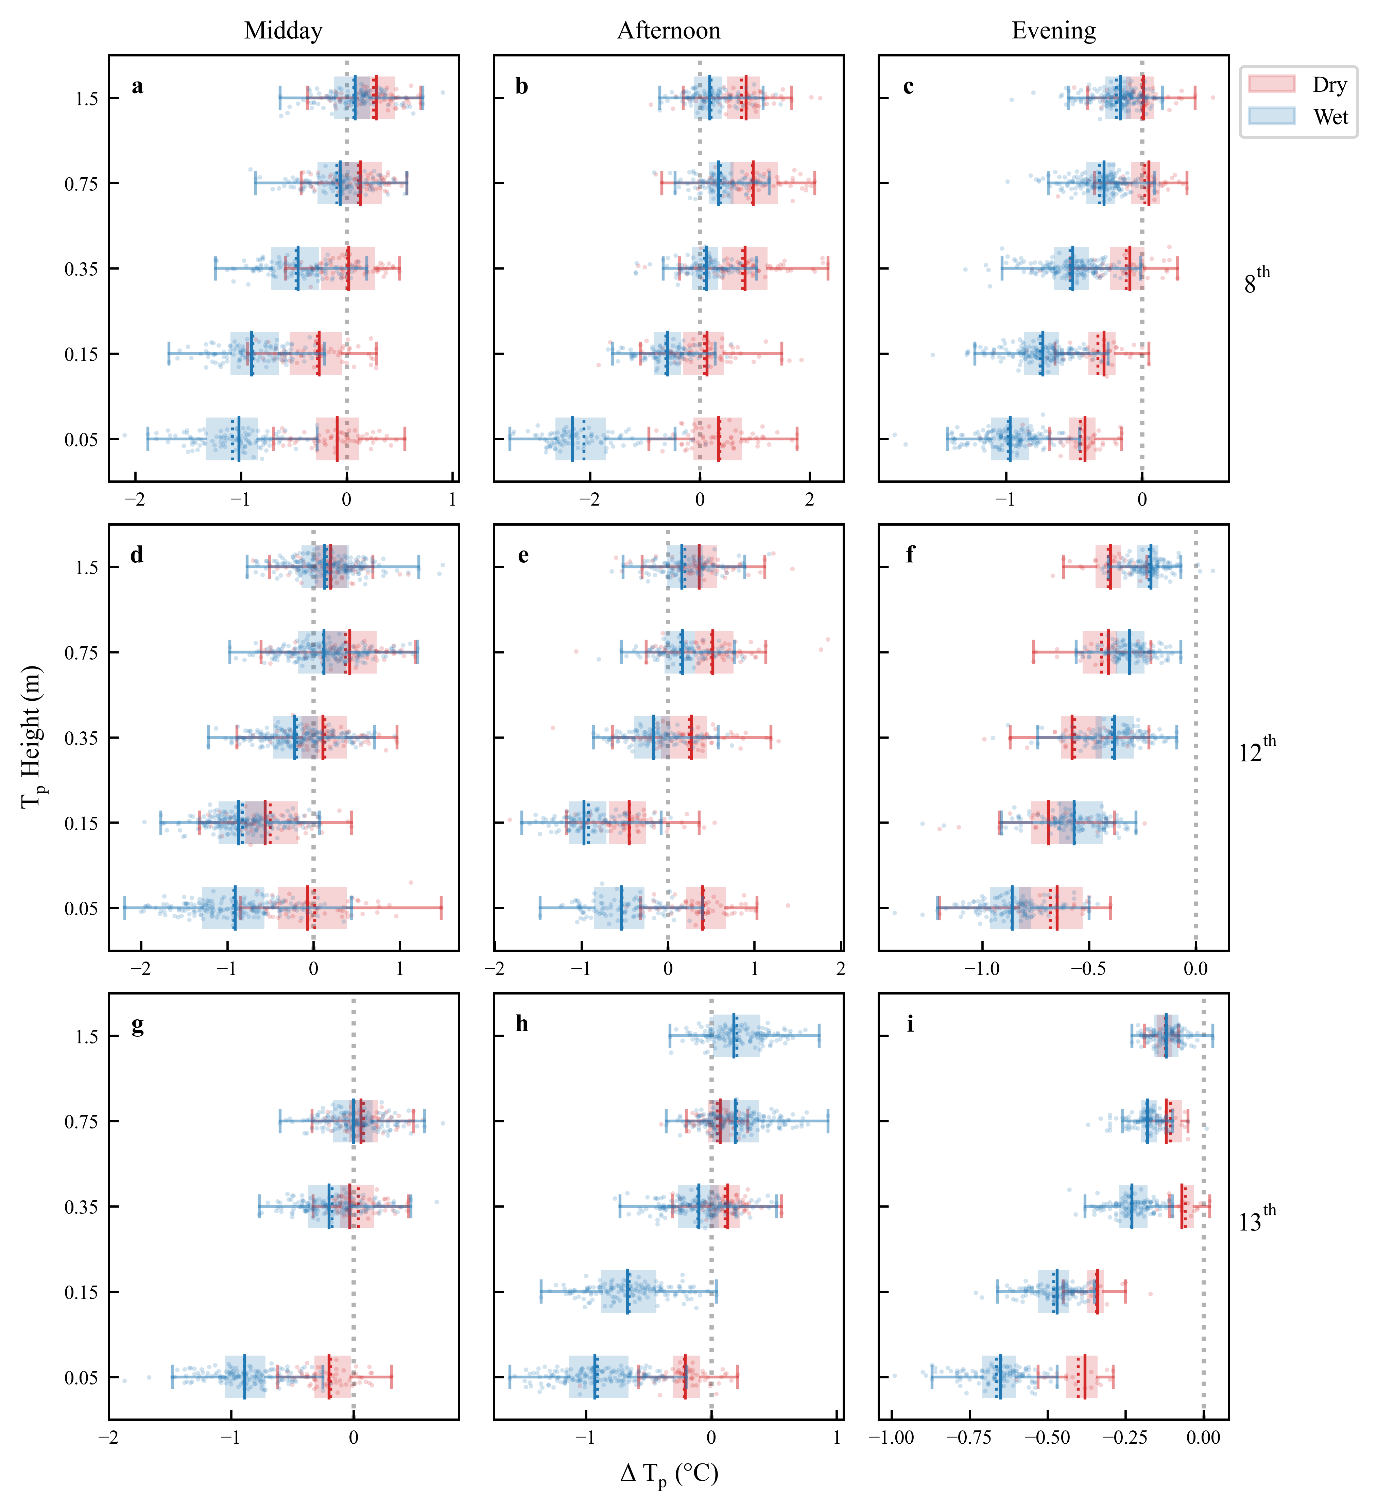
\includegraphics[trim={0 0 0 0},clip,scale=1.0]{pict038.png}
\caption{\bf Boxplots of the raw $\Delta$\gls{tp} for dry and wet periods of each experiment at each \gls{tp} height. Rows correspond to the experiment day; columns correspond to the experiment time category.}
 \label{fig:7.9}
\end{figure}

%\subsubsection{Temperature Profile $\Delta$ vs Control}\label{sec:appendix7.5.2}

\begin{figure}
\centering
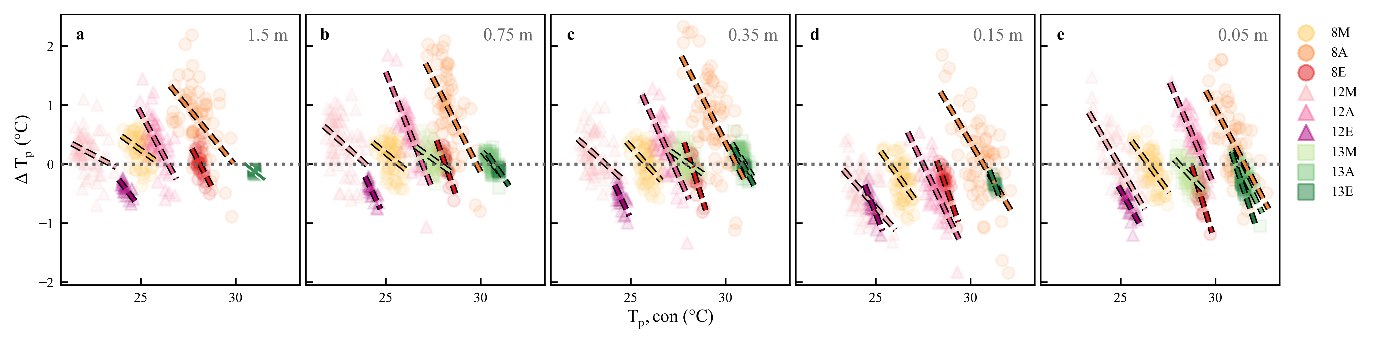
\includegraphics[trim={0 0 0 0},clip,scale=1.0]{pict039.png}
\caption{\bf $\Delta$\gls{tp} and \gls{tpcon} at each \gls{tp} height, lines showing the linear relationship for each experiment. The black outline indicates if the linear relationship is statistically significant (\gls{p} $<$ 0.05).}
 \label{fig:7.10}
\end{figure}



%\subsubsection{$\Delta$ Temperature Profile Control Correction}\label{sec:appendix7.5.3}
\begin{figure}
\centering
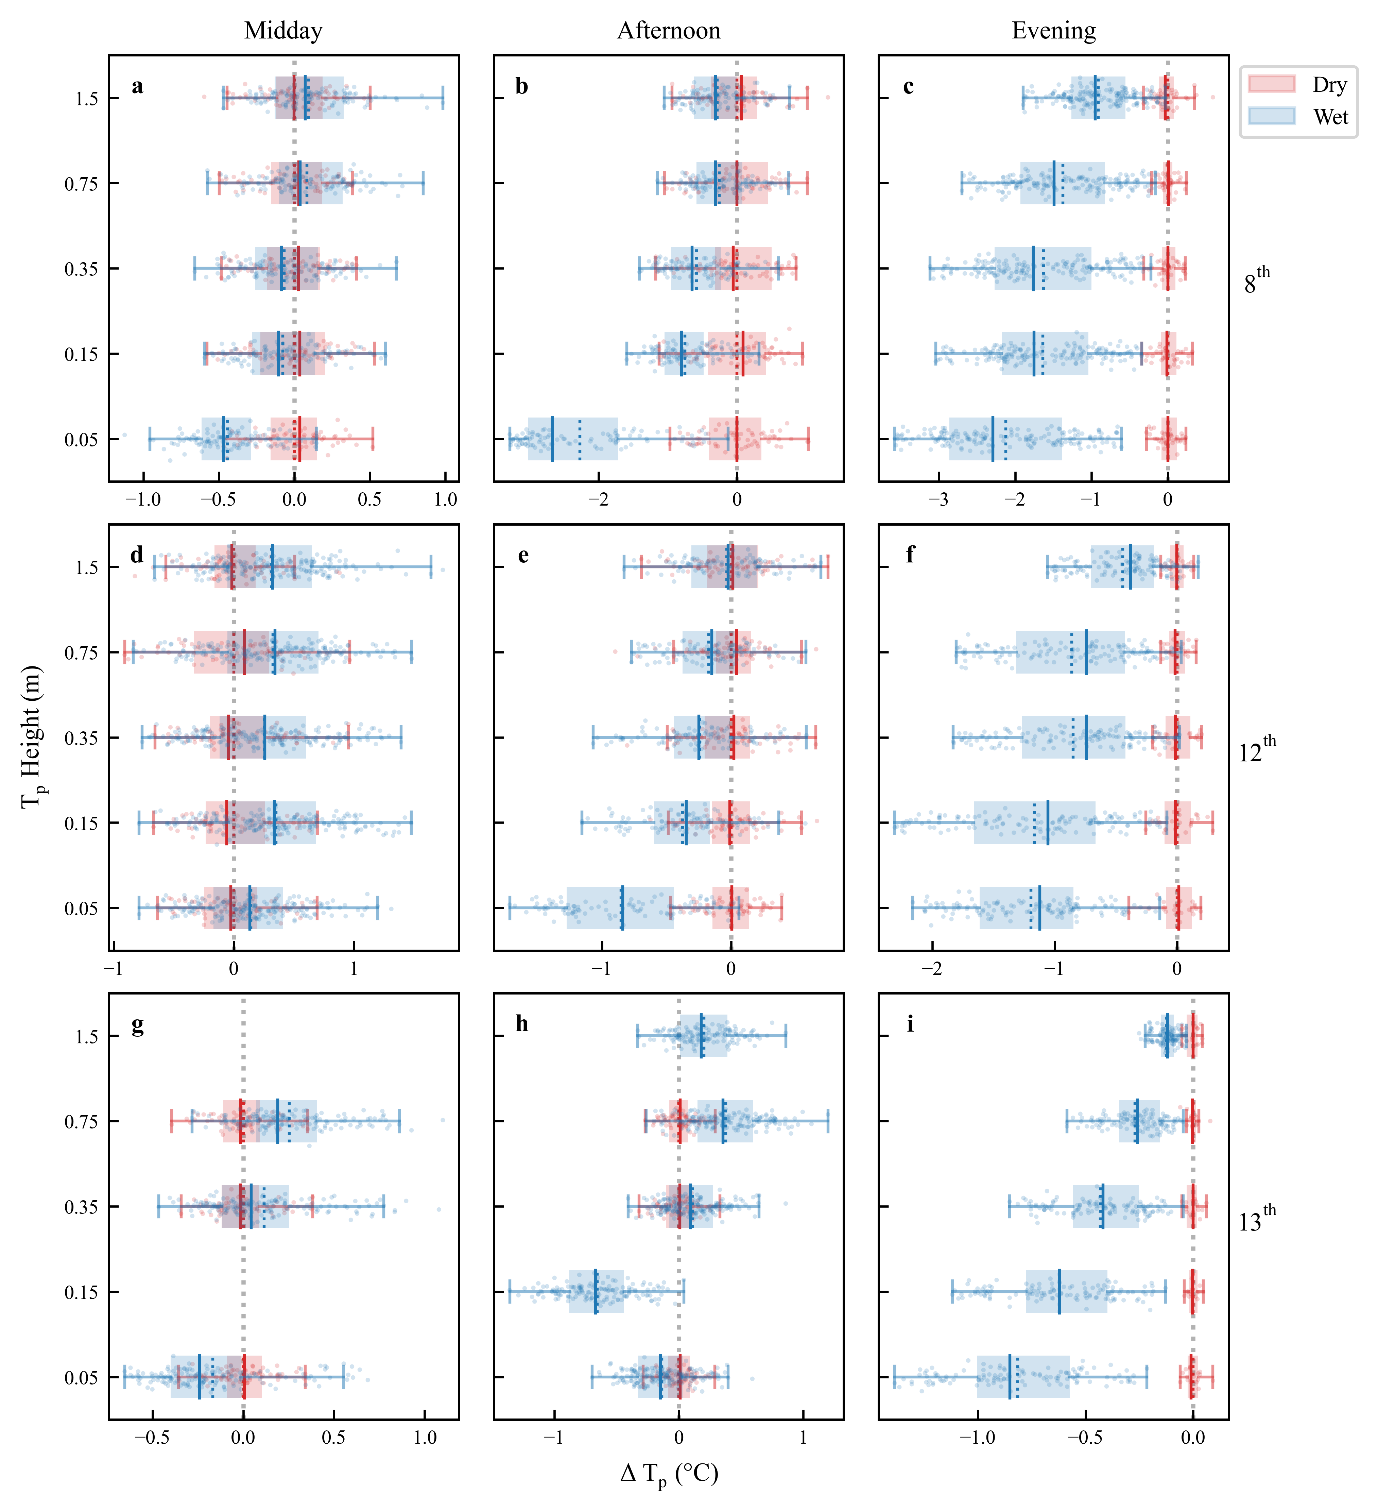
\includegraphics[trim={0 0 0 0},clip,scale=1.0]{pict040.png}
\caption{\bf Boxplots of the $\Delta$\gls{tp} for dry and wet periods of each experiment at each \gls{tp} height, corrected by detrending based on the linear relationship between $\Delta$\gls{tp} and \gls{tpcon} (Figure \ref{fig:7.10}). Rows correspond to the experiment day; columns correspond to the experiment time category.}
 \label{fig:7.11}
\end{figure}


%\subsubsection{Temperature Profile $\Delta$ vs Wind}\label{sec:appendix7.5.4}

\begin{figure}
\centering
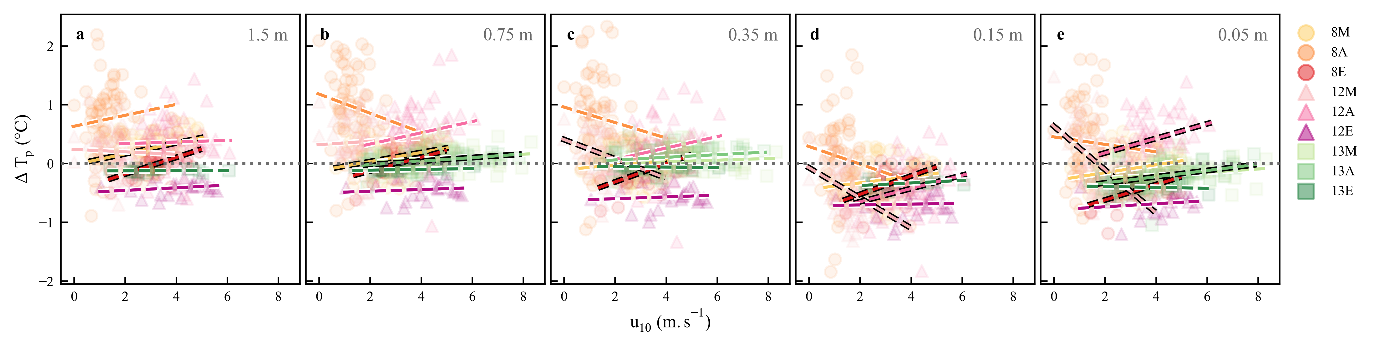
\includegraphics[trim={0 0 0 0},clip,scale=1.0]{pict041.png}
\caption{\bf $\Delta$\gls{tp} and \gls{u10} at each \gls{tp} height, lines showing the linear relationship for each experiment. The black outline indicates if the linear relationship is statistically significant (\gls{p} $<$ 0.05).}
 \label{fig:7.12}
\end{figure}


%\subsubsection{$\Delta$ Temperature Profile Wind Correction}\label{sec:appendix7.5.5}

\begin{figure}
\centering
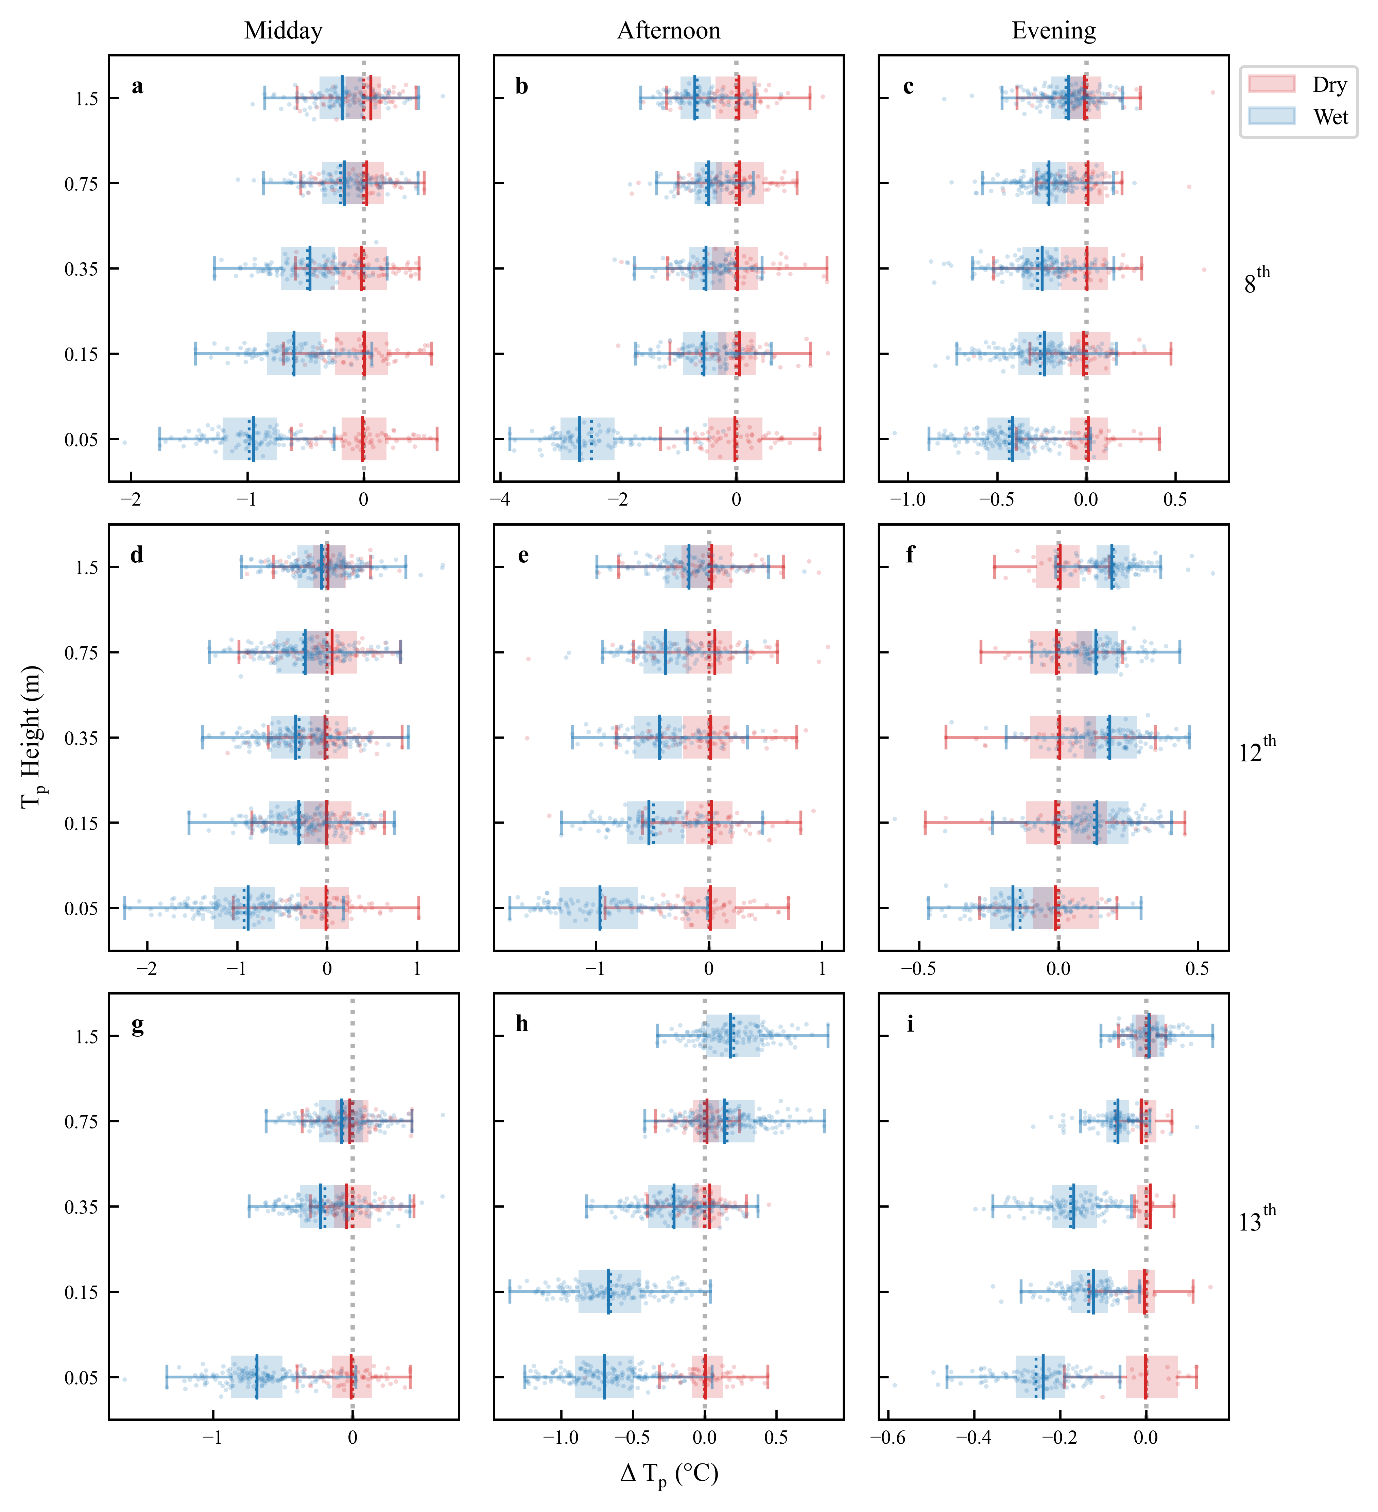
\includegraphics[trim={0 0 0 0},clip,scale=1.0]{pict042.png}
\caption{\bf Boxplots of the $\Delta$\gls{tp} for dry and wet periods of each experiment at each \gls{tp} height, corrected by detrending based on the linear relationship between $\Delta$\gls{tp} and \gls{u10} (Figure \ref{fig:7.12}). Rows correspond to the experiment day; columns correspond to the experiment time category.}
 \label{fig:7.13}
\end{figure}


%\subsubsection{$\Delta$ Temperature Profile Mean Adjustment}\label{sec:appendix7.5.6}

\begin{figure}
\centering
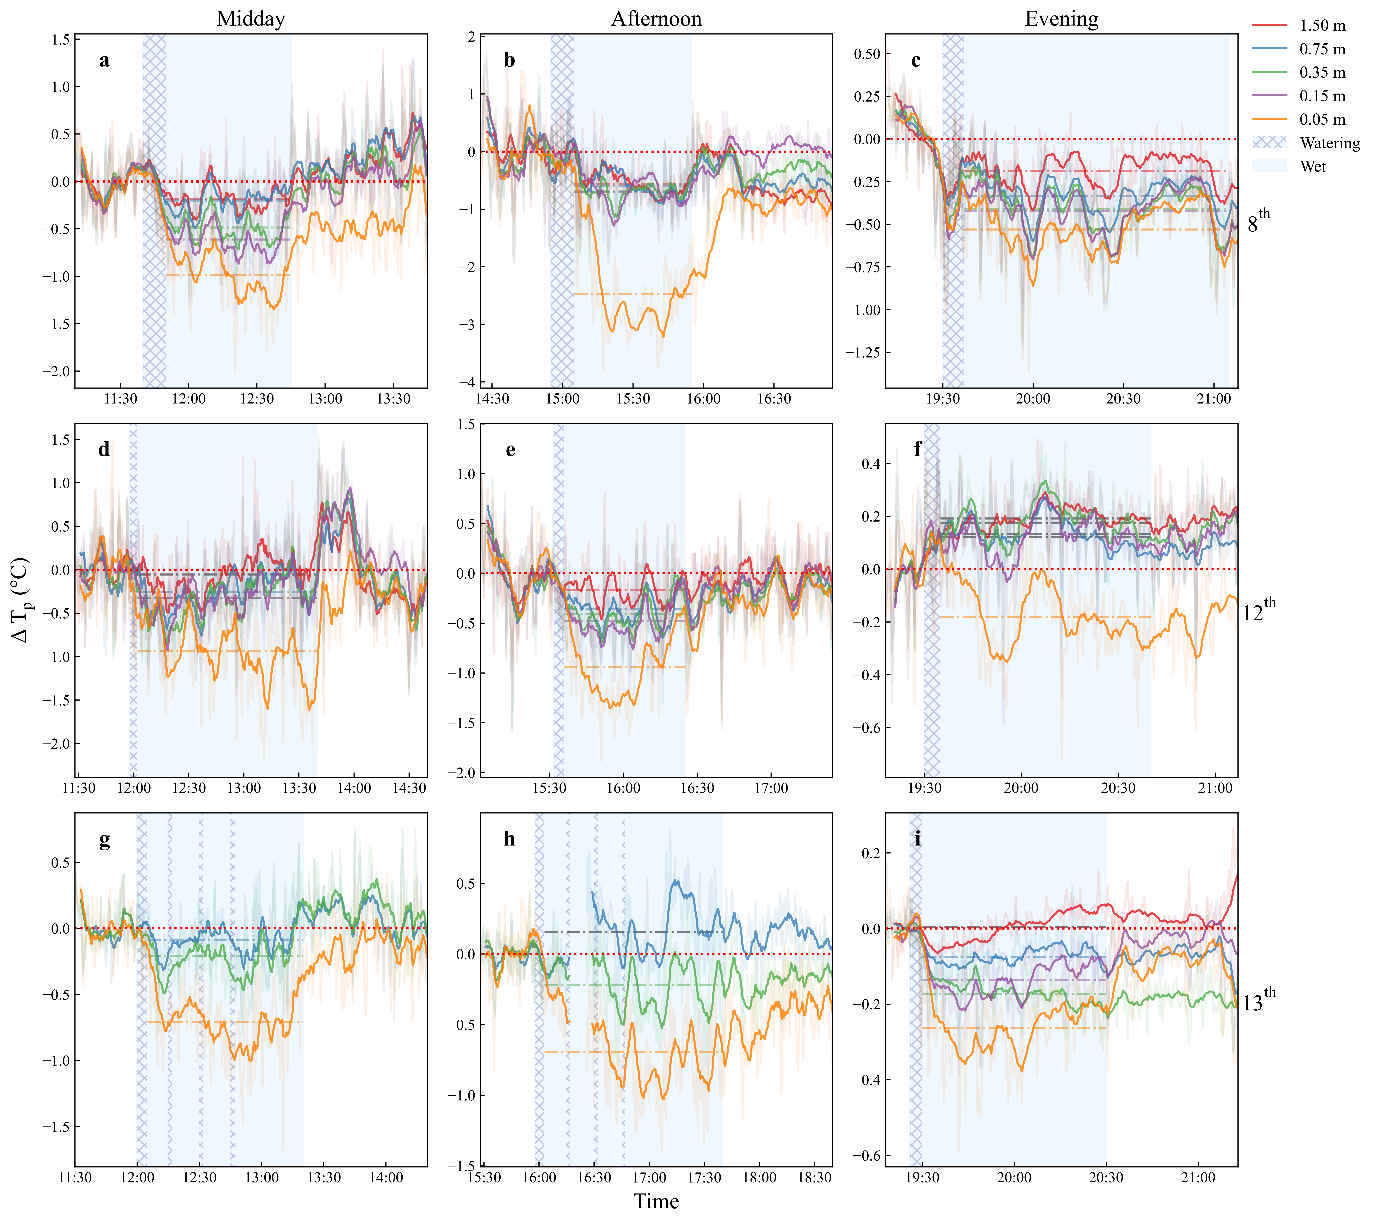
\includegraphics[trim={0 0 0 0},clip,scale=1.0]{pict043.png}
\caption{\bf $\Delta$\gls{tp} corrected based on the mean of before watering for each experiment. The transparent lines are the raw data, while the solid lines are the 5-minute running average. The dashed lines on (b) represented the mean of the wet period, where grey represents a statistically insignificant change (\gls{p} $>$ 0.05). Rows correspond to the experiment day; columns correspond to the experiment time category.}
 \label{fig:7.14}
\end{figure}


%\subsubsection{Pavement Watering Impact on Kestrel Temperature}\label{sec:appendix7.5.7}

\begin{table}[!ht]\caption{\gls{pwimpact} for \gls{Kt} for all experiments.}
    \centering
    \begin{tabular}{|l|l|}
    \hline
        Experiment & PWimpact for KT \\ \hline
        08M & -0.45 \\ \hline
        08A & +0.59 \\ \hline
        08E & -0.10 \\ \hline
        12M & -0.35 \\ \hline
        12A & -0.27 \\ \hline
        12E & -0.11 \\ \hline
        13M & +0.61 \\ \hline
        13A & -0.84 \\ \hline
        13E & -0.18 \\ \hline
    \end{tabular}\label{table:7.4}
\end{table}


%\subsubsection{Surface Temperature Transects Summary}\label{sec:appendix7.5.8}

\begin{figure}
\centering
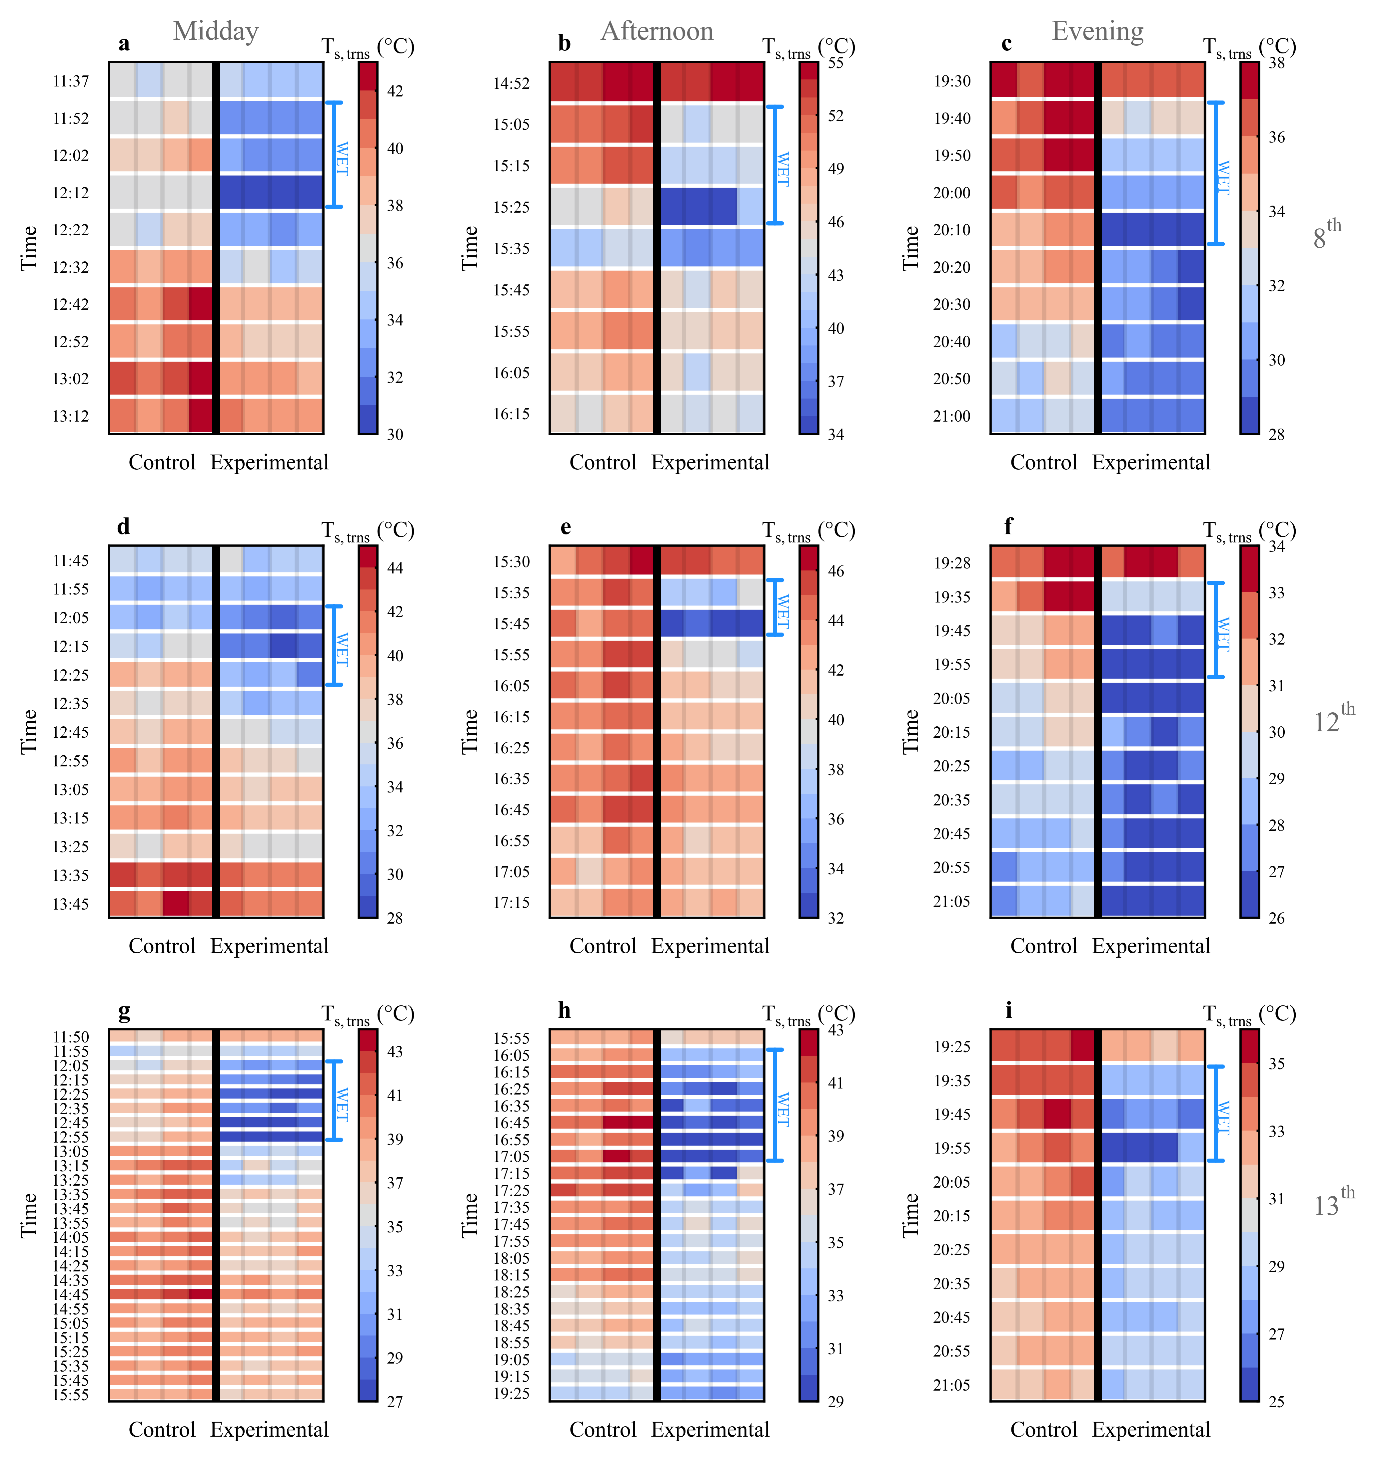
\includegraphics[trim={0 0 0 0},clip,scale=1.0]{pict044.png}
\caption{\bf The \gls{tstrns} of all experiments showing the evolution from before, during, and after the wet period (subplot rows) for control and experimental points along the transect (subplot columns). Rows correspond to the experiment day; columns correspond to the experiment time category.}
 \label{fig:7.15}
\end{figure}


%\subsubsection{$\Delta$ Surface Temperature Transects Adjusted}\label{sec:appendix7.5.9}

\begin{figure}
\centering
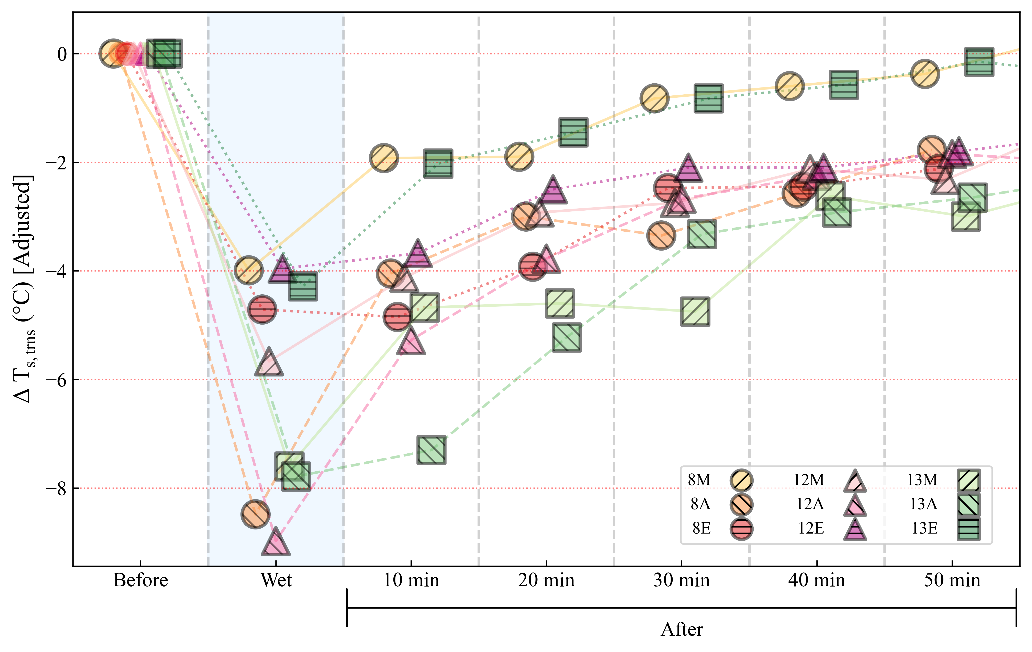
\includegraphics[trim={0 0 0 0},clip,scale=1.0]{pict045.png}
\caption{\bf The \gls{deltatstrns} of all experiments where the wet refers to the mean \gls{deltatstrns} of the wet period, adjusted so the before watering difference is zero. The black outline indicates that the experimental points are statistically significantly lower than the control points (\gls{p} $<$ 0.05).}
 \label{fig:7.16}
\end{figure}


%\subsubsection{Derived Surface Temperature}\label{sec:appendix7.5.10}

\begin{figure}
\centering
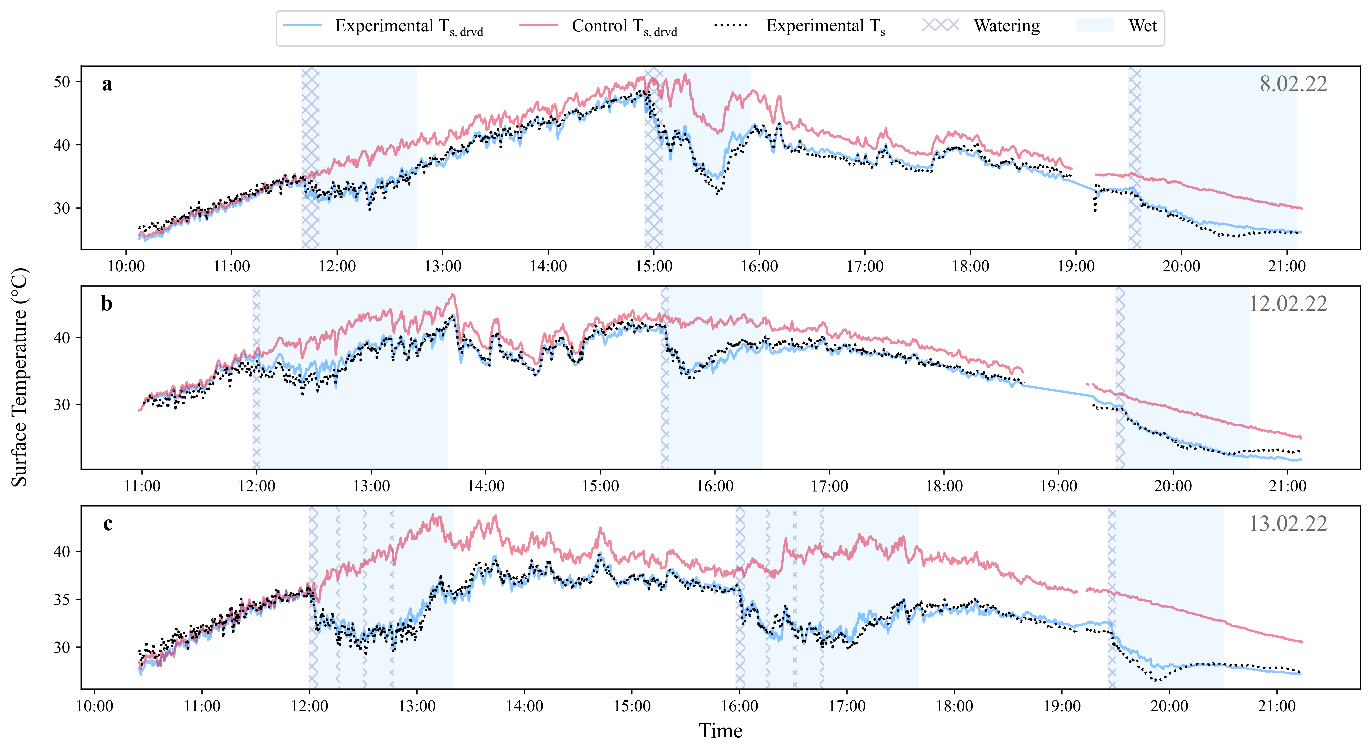
\includegraphics[trim={0 0 0 0},clip,scale=1.0]{pict028.png}
\caption{\bf \gls{tsdrvd} for the control and experimental site with \gls{ts} for the experiment days: (a) 8th, (b) 12th, (c) 13th.}
 \label{fig:7.17}
\end{figure}



\begin{table}[!ht]\caption{\gls{deltadry} and \gls{pwimpact} for \gls{tsdrvd} for all experiments.}
    \centering
    \begin{tabular}{|l|l|l|}
    \hline
        Experiment & \gls{deltadry} ($^{\circ}$C) &\gls{pwimpact} ($^{\circ}$C) \\ \hline
        08M & -0.46&-4.38 \\ \hline
        08A & -2.24&-5.10 \\ \hline
        08E & -2.42&-2.14 \\ \hline
        12M & -0.48&-3.25 \\ \hline
        12A & -1.77&-3.77 \\ \hline
        12E & -1.83&-2.49 \\ \hline
        13M & -0.25&-6.84 \\ \hline
        13A & -1.77&-5.53 \\ \hline
        13E & -3.37&-2.24 \\ \hline
    \end{tabular}\label{table:7.5}
\end{table}




%\subsubsection{Surface Energy Balance Before Watering}\label{sec:appendix7.5.11}

\begin{figure}
\centering
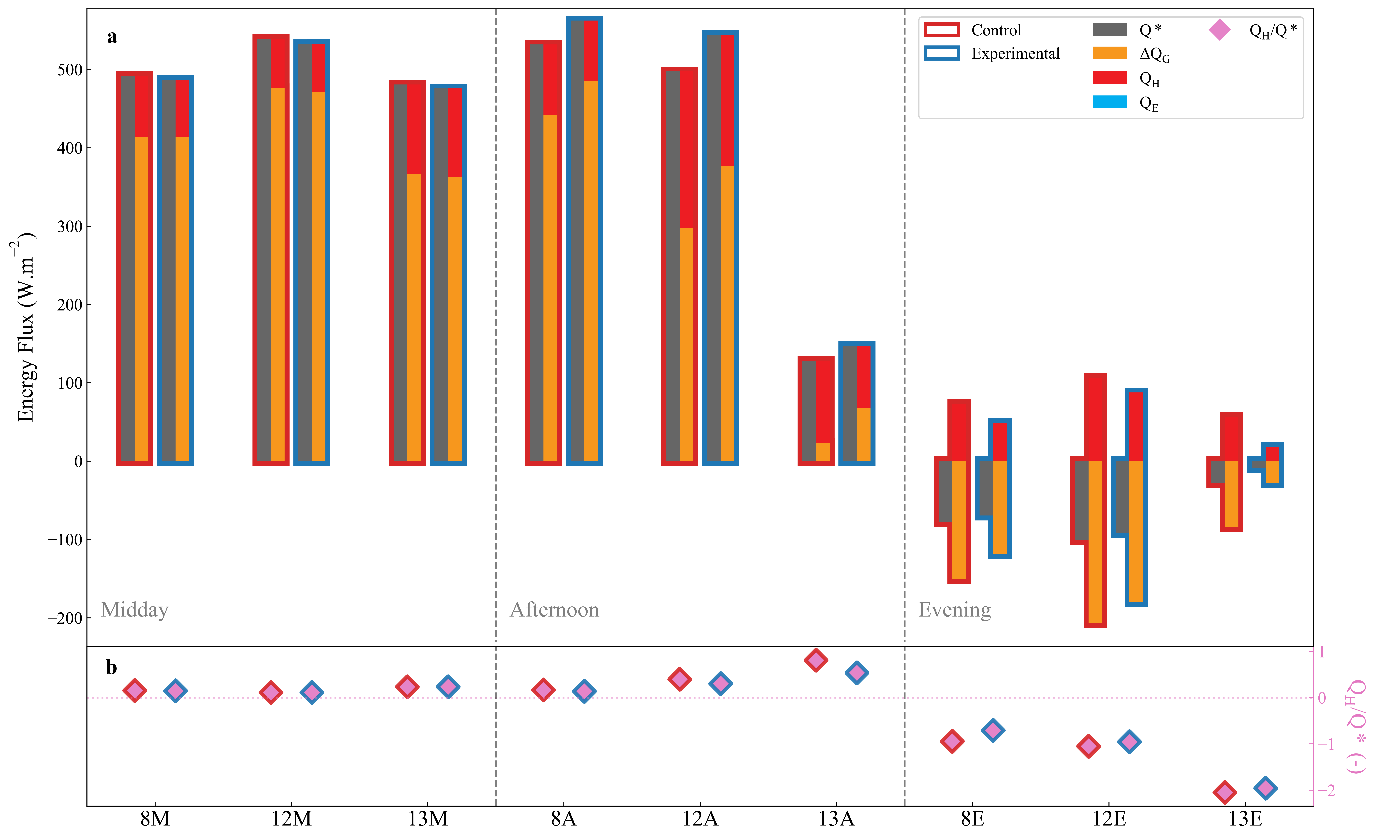
\includegraphics[trim={0 0 0 0},clip,scale=1.0]{pict046.png}
\caption{\bf (a) The mean surface energy balance of each experiment's control and experimental site before watering; (b) the \gls{Qh} and \gls{Qstar} ratio for each experiment.}
 \label{fig:7.18}
\end{figure}


%\subsubsection{Change in Sensible Heat Flux and Net Radiation Ratio}\label{sec:appendix7.5.12}

\begin{figure}
\centering
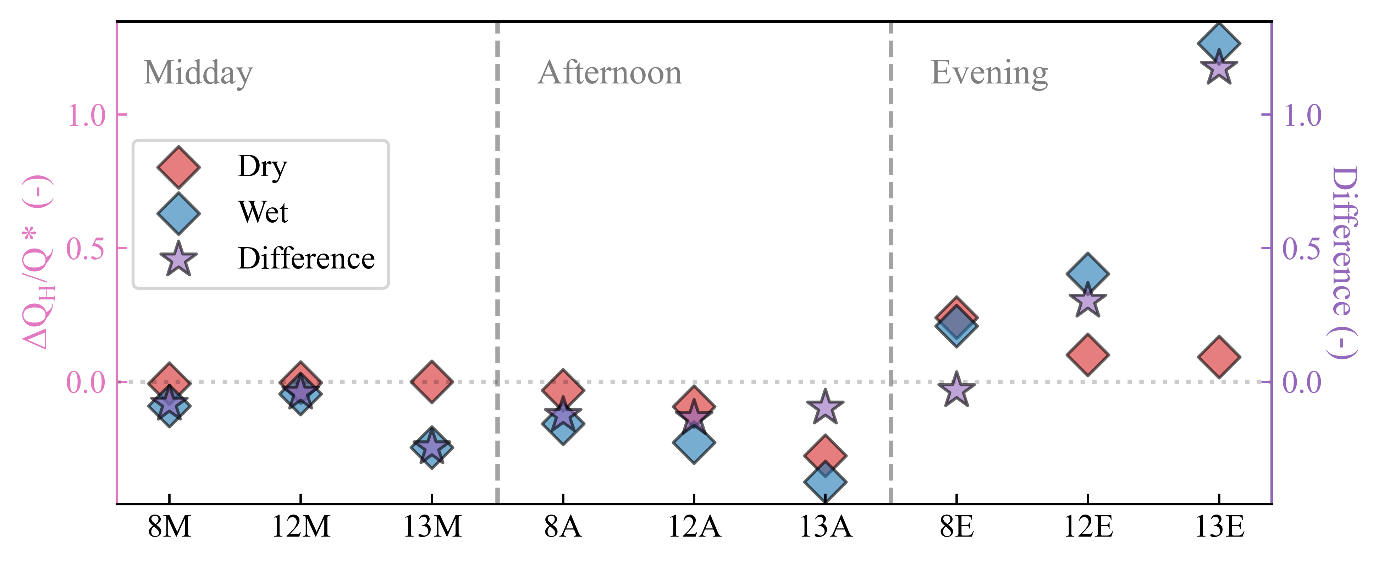
\includegraphics[trim={0 0 0 0},clip,scale=1.0]{pict047.png}
\caption{\bf The $\Delta$\gls{Qh}/\gls{Qstar} for the before watering (dry) and during wet (wet) time periods, along with their difference, for all experiments.}
 \label{fig:7.19}
\end{figure}s


%\section{Supplementary Figures}\label{sec:suppfig}
%\beginsupplement



\end{document}
